\documentclass[10pt,a4paper]{book}
\usepackage[utf8]{inputenc}
\usepackage[francais]{babel}
\usepackage[T1]{fontenc}
\usepackage{amsmath}
\usepackage{amsfonts}
\usepackage{amssymb}
\usepackage{graphicx}
\usepackage{tikz}
\usepackage[left=2cm,right=2cm,top=2cm,bottom=2cm]{geometry}
\usepackage[colorlinks=false,urlcolor=red]{hyperref}
\usepackage{amsthm}

\newtheorem{definition}{D\'efinition}
\newtheorem{exemple}{Exemple}
\newtheorem{remarque}{Remarque}
\newtheorem{proposition}{Proposition}

\def\gint{\displaystyle\int}


\author{Brachet Matthieu}
\title{Schémas compacts hermitiens - application en climatologie et océanographie numérique}

\graphicspath{{../Images/}}

\begin{document}

\maketitle
\newpage
\tableofcontents
\listoffigures


\section*{Introduction}
%%% *** INTRODUCTION ***************************************************************************

\section{Introduction}
\label{sec:1}
In this paper, we continue the development
of the compact scheme approach introduced in \cite{} and \cite{}
for hyperbolic problems on the sphere.
In recent years a lot of effort
has been devoted to import
ideas of numerical gas dynamics to numerical climatology.
Two particular examples are finite volumes upwind schemes 
with numerical fluxes. This approach involves
reconstruction with piecewise cubic recontsruction.
A variant is the Discontinuous Galerkin approach
in which several unknowns in a single computational cells are used.
In each of these two cases, the machinery of upwind schemes is adapted
to the specificity of the spherical context
and of the test cases. This involves in particular 
slope limiting. 

An important challenge for numerical schemes in numerical climatology 
is to calculate as accurately as possible 
the solution of linear equations up to a large physical time.
Here we show that our compact scheme performs well
for the three following problems:
\begin{itemize}
\item 
The linear scalar equation
advection 
\begin{equation}
\label{eq:adv}
\dfrac{\partial h}{\partial t}  (t,\mathbf{x})+ \mathbf{c}(t,\mathbf{x}) \cdot \nabla_T h(t,\mathbf{x})=0
\end{equation}

The velocity $\mathbf{c}(t,\mathbf{x}) \in (0, +\infty) \times \mathbb{S}^2$ is prescribed
so that the scalar value $h(t,\mathbf{x})$ exhibits a moving rollup vortex.
This test case was introduced
in \cite{Nair-Machenhauer,Nair-Jablonowski}. We refer to Sections
\ref{sec:4.1} and \ref{sec:4.2} for setails.
\item
The linearized shallow water equations (LSWE). This equation
is expressed as:
\begin{equation}
\label{eq:lswe}
(LSWE) \left\{
\begin{array}{l}
\dfrac{\partial \mathbf{v} }{\partial t} (t,\mathbf{x})+ g \nabla_T \eta(t,\mathbf{x}) + f(\mathbf{x}) \mathbf{k}(\mathbf{x}) \wedge
\mathbf{v}(t,\mathbf{x})=0\\
\dfrac{\partial \eta}{\partial t} (t,\mathbf{x})+ H \nabla_T \cdot \mathbf{v}(t,\mathbf{x})=0
\end{array}
\right.
\end{equation}


This system serves as a base for spherical waves on the sphere,
\cite{Paldor}. The state at rest is 
$(\mathbf{v}_0,\eta_0)=(0,H)$ and the 
The 3-components perturbation unknowns is
the vector $(t,\mathbf{x}) \mapsto (\mathbf{v}(t,\mathbf{x}), \eta(t,\mathbf{x}))$.
\item The shallow water equation (SWE). We use the vectorial form as following :
\begin{equation}
\label{eq:swe}
(SWE) \left\lbrace
\begin{array}{rcl}
\dfrac{\partial h^{\star}}{\partial t} (t,\mathbf{x}) + \nabla_T \cdot \left( h^{\star}(t,\mathbf{x}) \mathbf{v}(t,\mathbf{x}) \right) & = & 0 \\
\dfrac{\partial \mathbf{v}}{\partial t}  (t,\mathbf{x}) + \nabla_T \left( \dfrac{1}{2} \mathbf{v}(t,\mathbf{x})^2 + g h(t,\mathbf{x}) \right) + \left( f(\mathbf{x}) + \zeta(t,\mathbf{x}) \right) \mathbf{k}(\mathbf{x}) \wedge \mathbf{v}(t,\mathbf{x}) & = & \mathbf{0} 
\end{array}
\right.
\end{equation}

where $\zeta = \left( \nabla_T \wedge \mathbf{v} \right) \cdot \mathbf{k}$ is the relative vorticity. $h^{\star} = h - h_s$ with $h_s$ the reliefs map.
\end{itemize}

The present approach is related to compact scheme
approach. In this sense, it belongs 
to a classical approach, which can
be traced back to early works
in approximation and interpolation theory, \cite{Collatz}.

Two specific applications in CFD where compact schemes
are  is Aeroacoustics, \cite{Visbal-Gaitonde, Tam-Webb} and Turbulence, \cite{Lele, Kim-Moin}.

Finite difference schemes 
for simulating problems in climatology have
actually attracted interest since 
more than 40 years, \cite{Arakawa}.

In both cases, we show 
that our purely Cartesian approach supports
the comparison with modern conservative schemes on unstructured grids, such as 
Discontinuous Galerkin or Finite-Volume schemes.
Note finally that Finite Difference methods were recently used
in numerical climatology in \cite{Ghader-Nordstrom}.

The outline of the paper is as follows.
In Section \ref{sec:2}, we recall the numerical calculation
of the gradient introduced in \cite{Croisille-10}. Then in Section 
\label{sec:3}, we present the numerical scheme with emphasis 
on the role of the filtering. Dissipation and dispersion analysis 
is given. Finally in Section \ref{sec:4}, we present 
numerical results on two vortex advection problems mentionned above.
These results show the accuracy of our scheme.
The accuracy is comparable to conservative schemes such as DG schemes \cite{Nair-Jablonowski}.

%% SWE.tex

\chapter{Dérivation du modèle mathématique}

Le plan de ce chapitre sera probablement largement retouché par la suite.

\section{Cadre du problème}


\section{Système adimensionné}



\section{Equation Shallow Water}

\subsection{Approximation d'ordre 1}

\subsection{Approximation d'ordre 2}


% disc.tex
\chapter{Analyse numérique}

\section{Opérateur de filtrage }

\subsection{Opérateur de filtrage en dimension 1}

Lors de la discrétisation via un schéma aux différences finies et suite à la discrétisation en temps, des oscillations parasites du type "+1/-1" peuvent apparaître. Il s'agit de phénomènes haute fréquences qui peuvent provoquer des instabilités numériques. 

Si $\mathfrak{u}$ est une fonction de grille périodique, on note le filtre passe-bas $\mathcal{F}\mathfrak{u}$. Dans la pratique, nous cherchons $\mathcal{F}$ sous la forme 

\begin{equation}
\mathcal{F} = \gsum_{k=0}^F a_k \dfrac{\tau^k + \tau^{-k}}{2}
\label{eq:ftr}
\end{equation}

Les coefficients $(a_k)_{0 \leq k \leq F}$ sont déterminés de manière à supprimer les phénomènes oscillants hautes fréquences (figure \ref{fig:hf_waves}) de la formes $\mathfrak{u}$ avec 
\begin{equation}
\mathfrak{u}_j = (-1)^j
\end{equation}

\begin{figure}[htbp]
\begin{center}
\begin{tikzpicture}[scale=1.4]
	\draw (-4,1) -- (-3,-1) ;
	\draw (-3,-1) -- (-2,1) ;
	\draw (-2,1) -- (-1,-1) ;
	\draw (-1,-1) -- (0,1) ;
	\draw (0,1) -- (1,-1) ;
	\draw (1,-1) -- (2,1) ;
	\draw (2,1) -- (3,-1) ;
	\draw (3,-1) -- (4,1) ;
	
	\draw (4,0) -- (-4,0) ;
	\foreach \k in {-3,...,3}
		{\draw  (\k,0) node[color=blue] {$\bullet$} ;
	   	\draw (\k,0) node {$\circ$} ;
	   	}
\end{tikzpicture}
\end{center}
\caption{Ondes de type "+1/-1".}
\label{fig:hf_waves}
\end{figure}


En considérant cette fonction de grille, on cherche $(a_k)_{0\leq k \leq F}$ tels que $\mathcal{F} \mathfrak{u} = \mathfrak{0}$, soit :
\begin{equation}
\mathcal{F}\mathfrak{u}_i = \gsum_{k=0}^F a_k \dfrac{\mathfrak{u}_{i+k} + \mathfrak{u}_{i-k}}{2} = \gsum_{k=0}^F a_k  \dfrac{(-1)^{i+k} + (-1)^{i-k}}{2} = 0.
\end{equation}
Cette équation est équivalente à 
\begin{equation}
\gsum_{k=0}^F a_k (-1)^k = 0
\label{eq:ftr_ftrcond}
\end{equation}
La relation \eqref{eq:ftr_ftrcond} nous donne une condition alors qu'il y a $F+1$ paramètres à déterminer. Il reste $F$ degrés de libertés dans l'opérateur de filtrage. Le choix qui est fait est de maximiser l'ordre du filtrage de manière à perturber un minimum la donnée initiale tout en supprimant les ondes parasites.

Le filtre doit conserver les très basses fréquences, lorsque $\mathfrak{u} = \mathfrak{1}$, on doit alors $\mathcal{F}\mathfrak{u} = \mathfrak{1}$.
C'est à dire que les coefficients $(a_k)_{0 \leq k \leq F}$ vérifient la relation de consistance
\begin{equation}
\gsum_{k=0}^F a_k = 1
\label{eq:ftr_conscond}
\end{equation}

Enfin, on remarque que si $u : x \in \Omega \mapsto u(x) \in \mathbb{R}$ et si $u^*$ est la fonction de grille associée à $u$, alors on a 
\begin{equation}
\begin{array}{rcl}
u(x_i + kh) & = & u(x_i) + p k u'(x_j) + \cdots + \dfrac{(kh)^l}{l!}u^{(l)}(x_i) + \cdots +\dfrac{(kh)^{2F}}{2F!} u^{(2F)}(\xi_k)\\
u(x_i - kh) & = & u(x_i) - p k u'(x_j) + \cdots + \dfrac{(-kh)^l}{l!}u^{(l)}(x_i) + \cdots +\dfrac{(-kh)^{2F}}{2F!} u^{(2F)}(\eta_k)
\end{array}
\end{equation}
avec $\xi_k \in [x_i, x_i+kh]$ et $\eta_k \in [x_i-kh, x_i]$. Alors par combinaison linéaire en considérant \eqref{eq:ftr_conscond} vérifiée, 
\begin{equation}
\mathcal{F}u^* - u^* = \gsum_{l=1}^{2F-1} \gsum_{k=0}^F \dfrac{a_k}{2} \underbrace{\dfrac{(kh)^l + (-kh)^l}{l!}}_{=0 \text{ pour } l \text{ impair.}}u^{(l)}(x_i) + \gsum_{k=0}^F \dfrac{a_k}{2}\dfrac{(kh)^{2F}}{2F!} \left( u^{(2F)}(\xi_k) + u^{(2F)}(\eta_k) \right)
\end{equation}
Ainsi, la condition de précision est 
\begin{equation}
\gsum_{k=0}^F a_k k^{2l} = 0 \text{ pour } 1 \leq l \leq F-1.
\label{eq:ftr_prescond}
\end{equation}

\begin{theoreme}
Soit $F \in \mathbb{N}^{\star}$. Il existe un unique $(a_k)_{0 \leq k \leq F}$ tel que $\mathcal{F}$ soit à la fois consistant en vérifiant \eqref{eq:ftr_conscond}, précis en vérifiant \eqref{eq:ftr_prescond} et soit un filtre passe bas en satisfesant \eqref{eq:ftr_ftrcond}. L'erreur de troncature du filtre est alors donnée par 
\begin{equation}
\mathcal{F}u^* - u^* = h^{2F} \gsum_{k=0}^F \dfrac{a_k}{2} \dfrac{k^{2F}}{2F!} \left( u^{(2F)}(\xi_k) + u^{(2F)}(\eta_k) \right).
\end{equation}
\label{prop:filter_def}
\end{theoreme}

\begin{proof}
La forme de l'erreur de troncature a déjà été vue, il reste à prouver l'unicité.

Après avoir retiré \eqref{eq:ftr_ftrcond} à \eqref{eq:ftr_conscond}, dire qu'il existe une unique $(a_j)_{0 \leq j \leq J}$ satisfesant les conditions est équivalent à dire que la matrice

\begin{equation}
A=\begin{bmatrix}
1 &  1  &  1  &  1  &  1  &  1  & \cdots\\  
0 &  2  &  0  &  2  &  0  & 2  & \cdots\\
0 &  1  & 2^2 & 3^2 & 4^2 & 5^2 & \cdots\\
0 &  1  & 2^4 & 3^4 & 4^4 & 5^4 & \cdots\\
0 &  1  & 2^6 & 3^6 & 4^6 & 5^6 & \cdots\\
&&& \vdots &  \vdots &
\end{bmatrix} \in \mathcal{M}_{J+1} \left( \mathbb{R} \right)
\end{equation}
est inversible car $a = [a_0, a_1, \cdots, a_J]^T$ est solution de 
\begin{equation}
A a = e_1
\end{equation}
avec $e = [1,1/2, 0,\cdots,0]^T$. En développant la seconde ligne de $A$, on a
\begin{equation}
\det ( A ) = \begin{vmatrix} 
2  &  0  &  2  &  0  & 2  & \cdots\\
1  & 2^2 & 3^2 & 4^2 & 5^2 & \cdots\\
1  & 2^4 & 3^4 & 4^4 & 5^4 & \cdots\\
1  & 2^6 & 3^6 & 4^6 & 5^6 & \cdots\\
& & \vdots &  \vdots &
\end{vmatrix} = 2 \sum_{k=1}^{\lfloor\frac{F-1}{2}\rfloor} \Delta_{2k+1}
\end{equation}
avec $\Delta_k$ donné par
\begin{equation}
\Delta_k = \begin{vmatrix} 
1 & 2^2 & \cdots & (k-1)^2 & (k+1)^2 & \cdots\\
1 & 2^4 & \cdots & (k-1)^4 & (k+1)^4 & \cdots\\
1 & 2^6 & \cdots & (k-1)^6 & (k+1)^6 & \cdots\\
&&& \vdots &  \vdots &
\end{vmatrix} = \dfrac{((F-1)!)^2}{k^2} \begin{vmatrix} 
1 & 1 & \cdots & 1 & 1 & \cdots\\
1 & (2^2)^1 & \cdots & ((k-1)^2)^1 & ((k+1)^2)^1 & \cdots\\
1 & (2^2)^2 & \cdots & ((k-1)^2)^2 & ((k+1)^2)^2 & \cdots\\
&&& \vdots &  \vdots &
\end{vmatrix}
\end{equation}
On reconnait alors un déterminant de Van-Der-Monde, donc $\Delta_k = \prod_{1 \leq i < j \leq F-1} \left( \alpha_j - \alpha_i \right)$, avec 
\begin{equation}
\alpha_j = \left\lbrace
\begin{array}{ll}
j^2 & \text{ avec } 1 \leq j \leq k-1\\
(j+1)^2 & \text{ avec } k \leq j \leq J-2\\
\end{array}
\right.
\end{equation}
Alors si $i<j$, on a $\alpha_i < \alpha_j$, donc $\Delta_k>0$ et même $\det A$ est une somme de déterminants tous strictements positifs donc $\det A > 0$. $A$ est inversible et le résultat est prouvé.
\end{proof}
Quelques filtres particuliers sont donnés dans la table \ref{tab:filter} en fonction de leur ordre de précision.

\begin{table}[htbp]
\begin{center}
\begin{tabular}{|c||cccccc|}
\hline
\textbf{Ordre de précision} & $a_0$ & $a_1$ & $a_2$ & $a_3$ & $a_4$ & $a_5$ \\
\hline \hline
$2$ & $1/2$ & $1/2$ & & & & \\
\hline
$4$ & $10/16$ & $8/16$ & $-2/16$ & & & \\
\hline
$6$ & $44/64$ & $30/64$ & $-12/64$ & $2/64$ & & \\
\hline
$8$ & $186/256$ & $112/256$ & $-56/256$ & $16/256$ & $-2/256$ & \\
\hline
$10$ & $772/1024$ & $420/1024$ & $-240/1024$ & $90/1024$ & $-20/1024$ & $2/1024$ \\
\hline
\end{tabular}
\end{center}
\caption{Exemples de filtres de la forme \eqref{eq:ftr} et leurs ordres de précision.}
\label{tab:filter}
\end{table}

Dans la suite, nous supposerons que $(a_k)_{0 \leq k \leq F}$ satisfait les conditions \eqref{eq:ftr_conscond}, \eqref{eq:ftr_prescond} et \eqref{eq:ftr_ftrcond}.
Les valeurs propres et fonctions propres de $\mathcal{F}$ sont issues de la proposition \ref{prop:eigen_P(tau)}. Le résultat est immédiat.

\begin{theoreme}
Les valeurs propres de $\mathcal{F}$ sont données par $\beta^k$ avec 
\begin{equation}
\beta^k = \gsum_{f=0}^F a_k \cos \left( \dfrac{2 \pi k f}{N} \right)
\end{equation}
pour tout $0 \leq k \leq N-1$, $\beta^k$ est associé à la fonction propre $\mathfrak{u}^k$ telle que 
\begin{equation}
\mathfrak{u}^k_j = \exp \left[ i j \dfrac{2 \pi k}{N} \right].
\end{equation}
\end{theoreme}

On définit le \textit{symbole} du filtre $\mathcal{F}$ par la fonction $\beta : \theta \in [0, \pi] \mapsto \beta(\theta) \in \mathbb{R}$ donnée par :
\begin{equation}
\beta( \theta ) = \gsum_{f=0}^F a_k \cos \left( f \theta \right)
\end{equation}

\begin{proposition}
Il existe un unique polynôme $P$ de degré $F$ tel que 
\begin{equation}
\beta(\theta) = P(\cos \theta )
\end{equation}
De plus,
\begin{equation}
P(x) = 1 -\dfrac{1}{(-2)^F} (X - 1)^F.
\end{equation}
\end{proposition}

\begin{proof}
Soit $\theta \in [0, \pi]$, 
\begin{equation}
\beta(\theta) = \gsum_{f=0}^F a_f \cos \left( f \theta \right) = \gsum_{f=0}^F a_f T_f ( \cos \theta )
\end{equation}
où $T_f \in \mathbb{R}_f [X]$ est le $k-$ieme polynome de Tchebytchev. 
Ainsi il existe $P \in \mathbb{R}_F [x]$ tel que $\beta( \theta ) = P( \cos \theta )$. Ce polynôme est unique. Montrons que 
\begin{equation}
P(x) = 1 -\dfrac{1}{(-2)^F} (X - 1)^F.
\end{equation}
convient.

\begin{itemize}
\item on montre facilement que 
\begin{equation}
P( \cos 0 ) = 1 -\dfrac{1}{(-2)^F} (\cos 0 - 1)^F = 1,
\end{equation}
de même,
\begin{equation}
P( \cos \pi ) = 1 -\dfrac{1}{(-2)^F} (\cos \pi - 1)^F 1 -\dfrac{(-2)^F}{(-2)^F} = 0.
\end{equation}
\item On rappelle la formule de Fàa Di Bruno permettant de calculer la dérivée $n-$ième d'une composée. Si $f$ et $g$ sont des fonctions régulières, on a 
\begin{equation}
\dfrac{d^n}{dx^n} \left( f \circ g \right)(x) = \gsum_{k=1}^n f^{(k)}\left( g(x) \right) B_{n,k}\left( g'(x), g''(x), \cdots , g^{n-k+1}(x) \right)
\end{equation}
où $B_{n,k}$ est un polynôme de Bell. En utilisant cette formule avec $f = P$ et $g = \cos$, évaluée en $\theta = 0$, on montre que :
\begin{equation}
\dfrac{d^n}{d\theta^n} \left( P \circ \cos \right)(0) = \gsum_{k=1}^n P^{(k)}\left(1\right) B_{n,k}\left( -1,0,1,0, \cdots\right)
\end{equation}
Or, $P^{(k)}\left(1\right) = 0$ pour tout $k \geq 1$. Donc 
\begin{equation}
\dfrac{d^n}{d\theta^n} \left( P \circ \cos \right)(0) = 0
\end{equation}
\end{itemize}
Le polynôme $P$ convient et 
\begin{equation}
\beta( \theta ) = 1 - \dfrac{1}{(-2)^F}(\cos \theta -1)^F.
\end{equation}
\end{proof}

\begin{proposition}
Pour tout $\theta \in [0, \pi]$, on a 
\begin{equation}
0 \leq \beta ( \theta ) \leq 1
\end{equation}
\end{proposition}

\begin{proof}
Supposons qu'il existe $\theta \in [0, \pi]$ tel que $\beta(\theta) < 0$ ou $\beta(\theta) > 1$. Comme $\beta(0)=1$ et $\beta(\pi) = 0$, il existe $\tilde{\theta} \in ]0, \pi[$ tel que 
\begin{equation}
\beta'(\tilde{\theta}) = - \sin \tilde{\theta} P'(\cos \tilde{\theta} ) = 0
\end{equation}
Or $\sin \tilde{\theta} \neq 0$ pour $\tilde{\theta} \in ]0, \pi[$.
De plus, 
\begin{equation}
P'(X) = \dfrac{F}{(-2)^F}(X-1)^{F-1}
\end{equation}
donc en prenant $X = \cos \tilde{\theta}$,
\begin{equation*}
P'(X) = 0 \Leftrightarrow \cos \tilde{\theta} = 1
\end{equation*}
Ce qui est impossible pour $\tilde{\theta} \in ]0, \pi[$. Donc par l'absurde, le résultat est vérifié.
\end{proof}

La fonction $\beta$ permet de considérer le comportement du filtre sur les différentes fréquences $\theta \in [0, \pi]$. Les basses fréquences sont bien conservées alors que les hautes fréquences ($\theta$ proche de $\pi$) sont atténuées. Cette observation est visible sur la figure \ref{fig:freq_filter} représentant la fonction $\beta : \theta \mapsto \beta(\theta)$ associée aux filtres d'ordre 2, 4, 6, 8 et 10. 

\begin{figure}[htbp]
\begin{center}
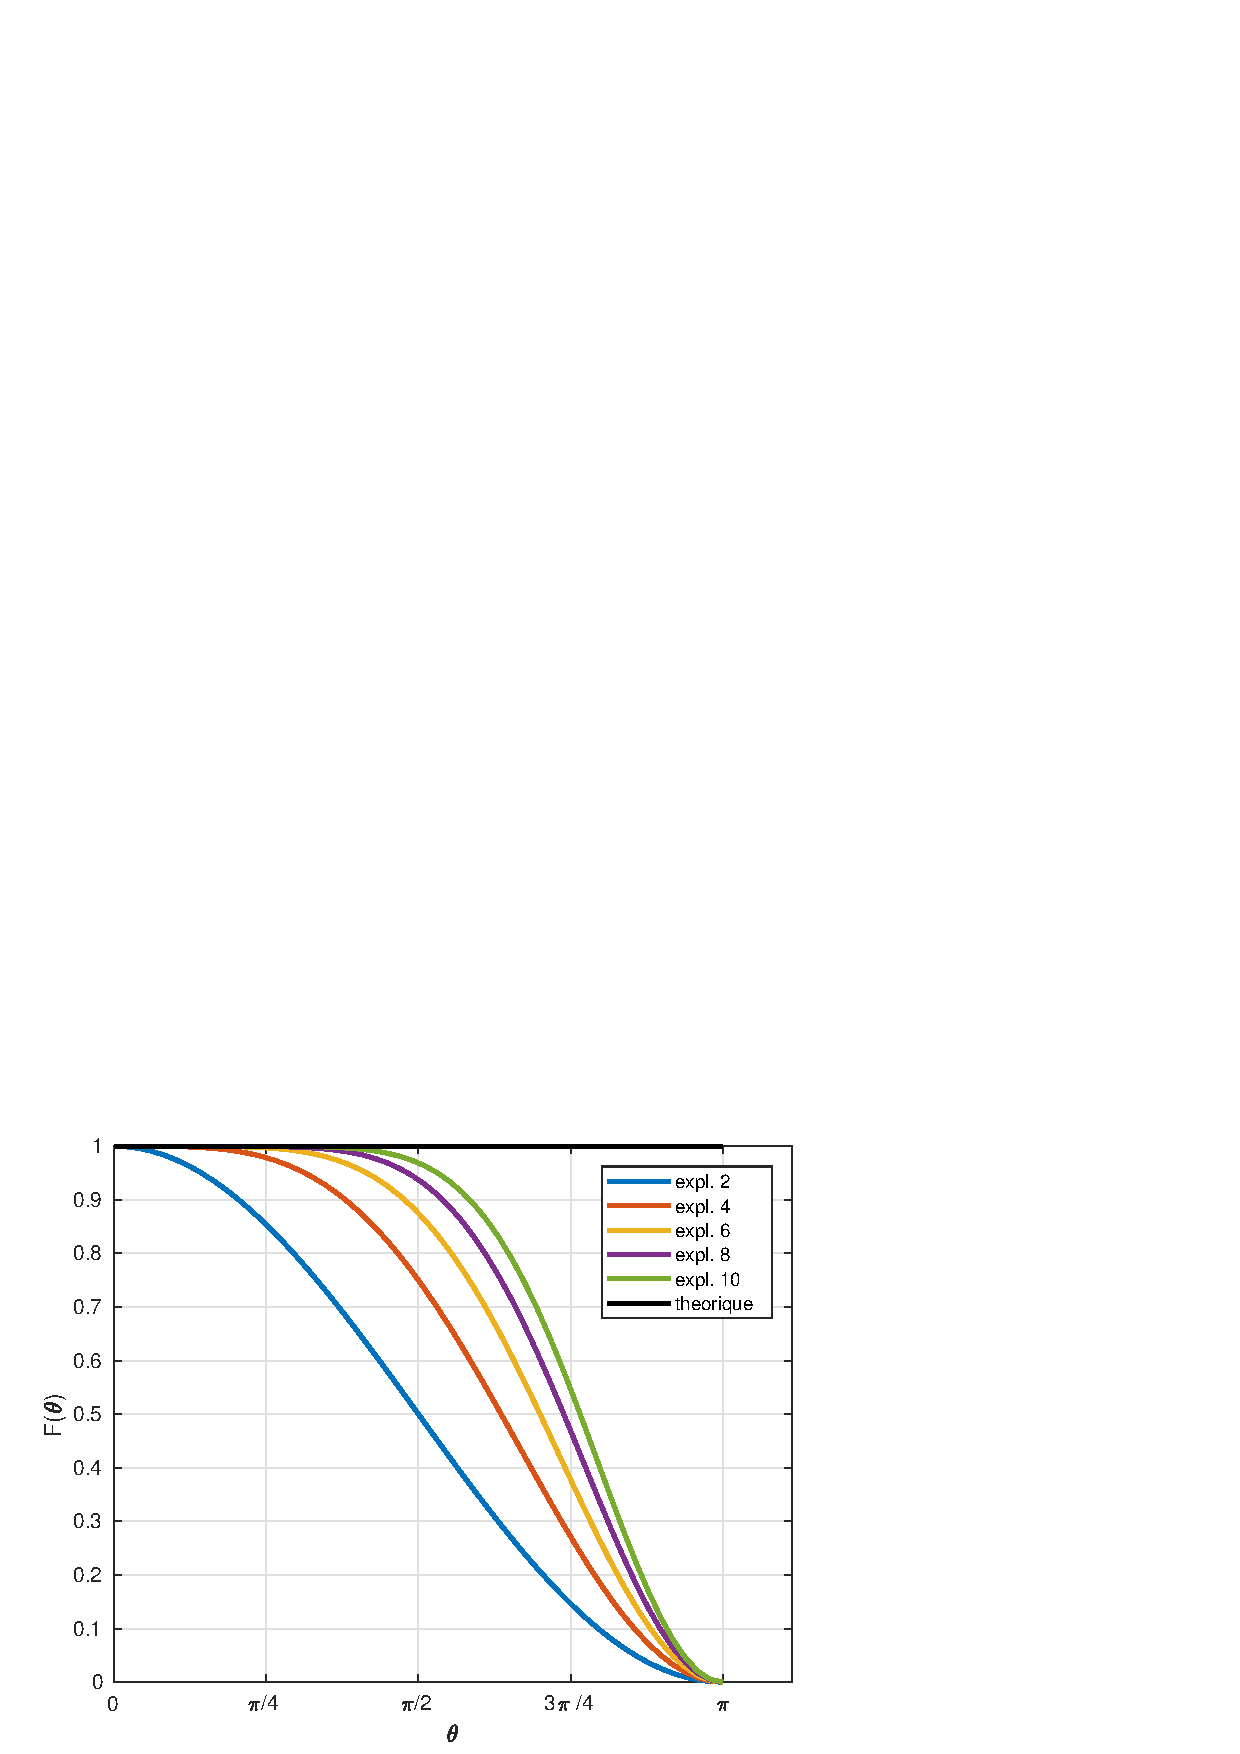
\includegraphics[scale=0.7]{freq_filter.png}
\end{center}
\caption{Fonction d'amplification $\beta$ pour les filtres explicites d'ordre 2, 4, 6, 8 et 10.}
\label{fig:freq_filter}
\end{figure}
Comme on s'y attendais, un filtre d'ordre élevé laisse passer un plus grand nombre de basses fréquences. Dans le tableau \ref{tab:filter_095}, on représente la fréquence $\theta_{0.95}$ maximale qui est conservée à $95\%$. Comme la fonction $\beta$ est strictement décroissante sur $[0,\pi]$, c'est une bijection de $[0,pi]$ dans $[0,1]$ et on a 
\begin{equation}
\theta_{0.95} = \beta^{-1}(0.95).
\end{equation}

\begin{table}
\begin{center}
\begin{tabular}{|c||c|}
\hline
\textbf{Ordre du filtre} & \textbf{Fréquence conservée à } $95\%$\\
\hline
\hline
$10$&$1.6695$\\
$8$&$1.5165$\\
$6$&$1.3045$\\
$4$&$0.9851$\\
$2$&$0.4510$\\
\hline
\end{tabular}
\end{center}
\caption{Fréquence conservée à $95\%$ en fonction de l'ordre du filtre.}
\label{tab:filter_095}
\end{table}

En pratique, cette fréquence $\theta_{0.95}$ est donnée en résolvant $\beta(\theta_{0.95})=0.95$ par 
\begin{equation}
\theta_{0.95} = \arccos \left[ 1-2 (0.05)^{1/F} \right].
\end{equation}
On remarque directement que la fonction $F \mapsto \theta_{0.95}$ est croissante, ce qui confirme que lorsque l'ordre de précision croit, $J$ croit et $\theta_{0.95}$ croit donc le filtre conserve un plus grand nombre de fréquences. De plus, 
\begin{equation}
\lim_{F \rightarrow \infty} \theta_{0.95} = \pi.
\end{equation}
Ce qui confirme la prise en compte d'un grand nombre de fréquence lorsque l'on augmente l'ordre du filtre. Cependant lorsque l'ordre du filtre augmente, l'effet de filtrage des hautes fréquences diminue.

Si $\mathfrak{u}$ est une fonction de grille, on pose $U$ et $\tilde{U}$ les vecteurs de $\mathbb{R}^N$ tel que
\begin{equation}
U = \begin{bmatrix}
\mathfrak{u}_1\\
\mathfrak{u}_2\\
\vdots \\
\mathfrak{u}_N\\
\end{bmatrix} \text{ et } 
\tilde{U} = \begin{bmatrix}
\mathcal{F}\mathfrak{u}_1\\
\mathcal{F}\mathfrak{u}_2\\
\vdots \\
\mathcal{F}\mathfrak{u}_N\\
\end{bmatrix}
\end{equation}
Alors $U$ et $\tilde{U}$ vérifient la relation
\begin{equation}
\tilde{U} = M F
\end{equation}
avec $M \in \mathcal{M}_N \left( \mathbb{R} \right)$ la matrice associée au filtrage des données en dimension 1 (dans le cas $F=2$):
\begin{equation}
M = \dfrac{1}{2}
\begin{bmatrix}
2a_0 & a_1 & a_2 &   &   &   & a_2 & a_1 \\ 
a_1 & 2 a_0 & a_1 & a_2 &   &   &   & a_2 \\ 
a_2 & a_1 & 2a_0 & a_1 & a_2 & (0) &   &   \\ 
  & a_2 & a_1 & 2a_0 & a_1 & a_2 &   &   \\ 
  &   & \ddots & \ddots & \ddots & \ddots & \ddots &   \\ 
  &   & (0) & a_2 & a_1 & 2 a_0 & a_1 & a_2 \\ 
a_2 &   &   &   & a_2 & a_1 & 2a_0 & a_1 \\ 
a_1 & a_2 &   &   &   & a_2 & a_1 & 2a_0
\end{bmatrix} 
\end{equation}
ou plus généralement 
\begin{equation}
M_{i,j} = \left\lbrace
\begin{array}{cl}
a_0 & \text{ si } i=j \\
\dfrac{1}{2} a_k & \text{ si } i+j \equiv k [N]\\
0 & \text{ sinon.}
\end{array}
\right.
\end{equation}
Il est clair que la matrice $M$ est symétrique.








\subsection{Opérateur de filtrage en géométrie cartésienne 2D}

Dans cette partie, nous utilisons toujours les notations de la section \ref{sec:notation_2D} en contexte périodique. Définissons les opérateurs de filtrage dans les directions $x$ et $y$ par
\begin{eqnarray*}
\mathcal{F}_x = \gsum_{k=0}^F a_k \dfrac{\tau_x^k + \tau_x^{-k}}{2} \\
\mathcal{F}_y = \gsum_{k=0}^F a_k \dfrac{\tau_y^k + \tau_y^{-k}}{2} \\
\end{eqnarray*}

Avec $(a_k)_{0 \leq k \leq F}$ vérifiant \ref{prop:filter_def}. Comme la géométrie est cartésienne, on remarque que 
\begin{equation}
\mathcal{F}_x \circ \mathcal{F}_y = \mathcal{F}_y \circ \mathcal{F}_x.
\end{equation}
Ce qui est faux lorsque la métrique n'est pas orthogonale.
La proposition \ref{prop:filter_def} permet de vérifier la consistance des opérateurs de filtrages.
Si $u : (x,y) \in \Omega \mapsto u(x,y) \in \mathbb{R}$ est fonction de $\mathcal{C}^{2F}$ alors :
\begin{eqnarray*}
\mathcal{F}_x u^*_{i,j} - u^*_{i,j} & = & C_xh^{2F}\\
\mathcal{F}_y u^*_{i,j} - u^*_{i,j} & = & C_yh^{2F}
\end{eqnarray*}
où $C_x$ et $C_y$ sont des constantes indépendantes de $h$.
En particulier, en composant les opérateurs, on peut définir un nouvel opérateur de filtrage. En effet  
\begin{equation}
(\mathcal{F}_x \circ \mathcal{F}_y) u_{i,j}^* - u_{i,j}^* = Ch^{2F}.
\end{equation}

L'écriture matricielle de l'opérateur de filtrage est donnée par la proposition suivante :
\begin{proposition}
Soit $\mathbf{u}$ une fonction de grille. Alors les opérateurs de filtrages s'écrivent à l'aide de matrices comme :
\begin{equation}
\left\lbrace
\begin{array}{rcl}
\text{vec}_2 (\mathcal{F}_x \mathbf{u}) & = & (Id \otimes M) \text{vec}_2 (\mathbf{u})\\
\text{vec}_2 (\mathcal{F}_y \mathbf{u}) & = & (M \otimes Id) \text{vec}_2 (\mathbf{u})\\
\end{array}
\right.
\end{equation}
\end{proposition}
Comme la matrice $M$ est symétrique, il est immédiat que $Id \otimes M$ et $M \otimes Id$ sont symétriques aussi.
















\section{Discrétisation temporelle}

\subsection{Discrétisation de Runge-Kutta d'ordre 4}

\subsection{Stabilité}

\subsection{Schéma filtré}















\section{Equation d'advection 1D}

\subsection{Discrétisation}

\subsection{Consistance et Stabilité}

\subsection{Relations de conservations}
% CS.tex
\chapter{Cubed-Sphere}

\section{Construction}

\section{Coordonnées}

\subsection{Tenseur métrique}

\subsection{Symboles de Christophel}
% opsph.tex
% opérateurs sphériques sur la sphère

\chapter{Approximation des opérateurs sphériques sur la Cubed-sphere}

La résolution des équations de type Shallow-Water \REF la sphère $\mathbb{S}_a^2$ demande le calcul approché d'opérateurs classiques. Les opérateurs différentiels sont indispensables pour la discrétisation spatiale. On pense en particulier aux opérateurs divergence, gradient ou rotationnel. Dans cette section, nous les définissons sur la Cubed-sphere. 
Nous avons vu dans le cas 1D qu'un opérateur de filtrage peut être utile pour supprimer les modes de type "$+1/-1$" qui perturbent le calcul lors de la discrétisation en temps. Nous définissons les opérateurs de filtrages permettant d'aboutir au filtrage qui sera utilisé dans la discrétisation temporelle des équations.
Dans ce chapitre, les notations employées telles que $\xi$, $\eta$, $\alpha$, ... sont celles employées dans le chapitre \REF concernant la Cubed-sphere.

\section{Opérateurs différentiels sur la Cubed-sphere}

\subsection{Définition des opérateurs}
Soit $\mathbf{x}_{i,j}^k$ un point de la Cubed-sphere avec $- N/2 \leq i,j \leq N/2$ et $k = (I) \cdots (VI)$. Alors il existe deux grands cercles $C_i^{(1)}$ et $C_j^{(2)}$ tels que $\mathbf{x}_{i,j}^k \in C_i^{(1)} \cap C^{(2)}_j$. $\alpha$ et $\beta$ sont respectivement les angles paramétrant $C_i^{(1)}$ et $C_j^{(2)}$.

On a définit le gradient en $\mathbf{x}_{i,j}^k$ par 
\begin{equation}
\nabla_T h = \dfrac{\partial h}{\partial \alpha}_{|C^{(2)}_j} \mathbf{g}^{\alpha} + \dfrac{\partial h}{\partial \beta}_{|C^{(1)}_i} \mathbf{g}^{\beta},
\end{equation}
où $h : \mathbf{x} \in \mathbb{S}_a^2 \mapsto h(\mathbf{x})$ est une fonction régulière sur la sphère.

Le cercle $C_i^{(1)}$ (resp. $C_j^{(2)}$) est une isocline $\xi = \xi_i$ (resp $\eta = \eta_j$) constant. D'après le théorème \eqref{th:gradient_xieta}, le gradient est 
\begin{equation}
\nabla_T h = \dfrac{\partial h}{\partial \xi}_{|\eta_j} \mathbf{g}^{\xi} + \dfrac{\partial h}{\partial \eta}_{|\xi_i} \mathbf{g}^{\eta}.
\end{equation}
On remarque que si l'on est capable de calculer les dérivées partielles $\partial_{\xi}$ et $\partial_{\eta}$ le long des grands cercles, alors on est capable de déterminer la valeur du gradient.

Soit $\mathbf{v} : \mathbf{x} \in \mathbb{S}_a^2 \mapsto \mathbf{v}(\mathbf{x}) \in \mathbb{T}_{\mathbf{x}} \mathbb{S}_a^2$ un champ de vecteur tangent à la sphère. On définit la \textit{divergence} et le \textit{rotationnel} de $\mathbf{v}$ notés $\nabla_T \cdot \mathbf{v}$ et $\nabla_T \wedge \mathbf{v}$.

\begin{definition}
Soit $\mathbf{v} : \mathbf{x} \in \mathbb{S}_a^2 \mapsto \mathbf{v}(\mathbf{x}) \in \mathbb{T}_{\mathbf{x}} \mathbb{S}_a^2$ un champ de vecteur régulier sur la sphère. Alors la divergence de $\mathbf{v}$ en $\mathbf{x} \in C_i^{(1)} \cap C_j^{(2)}$ est donnée par
\begin{equation}
\nabla_T \cdot \mathbf{v} = \dfrac{\partial \mathbf{v}}{\partial \alpha}_{|C^{(2)}_j} \cdot \mathbf{g}^{\alpha} + \dfrac{\partial \mathbf{v}}{\partial \beta}_{|C^{(1)}_i} \cdot \mathbf{g}^{\beta}.
\end{equation}
\label{def:divergence}
La notation $\cdot$ désigne le produit scalaire usuel dans $\mathbb{R}^3$.
\end{definition}
Le rotationnel d'un champ de vecteurs représente la tendance des lignes de courant de $\mathbf{v}$ à tourner autour d'un point. Il est définit par

\begin{definition}
Soit $\mathbf{v} : \mathbf{x} \in \mathbb{S}_a^2 \mapsto \mathbf{v}(\mathbf{x}) \in \mathbb{T}_{\mathbf{x}} \mathbb{S}_a^2$ un champ de vecteur régulier sur la sphère. Alors le rotationnel de $\mathbf{v}$ en $\mathbf{x} \in C_i^{(1)} \cap C_j^{(2)}$ est donnée par
\begin{equation}
\nabla_T \wedge \mathbf{v} =  \mathbf{g}^{\alpha} \wedge \dfrac{\partial \mathbf{v}}{\partial \alpha}_{|C^{(2)}_j} + \mathbf{g}^{\beta} \wedge \dfrac{\partial \mathbf{v}}{\partial \beta}_{|C^{(1)}_i}
\end{equation}
où $\wedge$ désigne le produit vectoriel.
\label{def:rotationnel}
\end{definition}
La \textit{vorticité} du champ de vecteurs $\mathbf{v}$ est la composante normale du rotationnel :
\begin{equation}
\vort ( \mathbf{v} ) = \left( \nabla_T \wedge \mathbf{v} \right) \cdot \mathbf{k}
\label{eq:vorticité}
\end{equation}
avec $\mathbf{k}$ le vecteur unitaire extérieur à la sphère en $\mathbf{x} \in \mathbb{S}_a^2$, vérifiant l'égalité
\begin{equation}
\mathbf{k} = \dfrac{1}{a} \mathbf{x}.
\end{equation}

En utilisant la proposition \ref{prop: g_alpha g_beta fct de g_xi g_eta}, il est facile de montrer que des égalités permettant de calculer les opérateurs à l'aide des dérivées en $\xi$ et en $\eta$.

\begin{theoreme}
Soit $h : \mathbf{x} \in \mathbb{S}_a^2 \mapsto h(\mathbf{x})$ une fonction régulière et $\mathbf{v} : \mathbf{x} \in \mathbb{S}_a^2 \mapsto \mathbf{v}(\mathbf{x}) \in \mathbb{T}_{\mathbf{x}} \mathbb{S}_a^2$ un champ de vecteurs régulier. Alors en $\mathbf{x}_{i,j}^k$ un point de la Cubed-Sphere, les égalités suivantes sont satisfaites :
\begin{itemize}
\item \textbf{Gradient} :
\begin{equation}
\nabla_T h = \dfrac{\partial h}{\partial \xi}_{|\eta_j} \mathbf{g}^{\xi} + \dfrac{\partial h}{\partial \eta}_{|\xi_i} \mathbf{g}^{\eta},
\end{equation}

\item \textbf{Divergence} :
\begin{equation}
\nabla_T \cdot \mathbf{v} = \dfrac{\partial \mathbf{v}}{\partial \xi}_{|\eta_j} \cdot \mathbf{g}^{\xi} + \dfrac{\partial \mathbf{v}}{\partial \eta}_{|\xi_i} \cdot \mathbf{g}^{\eta},
\label{eq:divergence_v1}
\end{equation}

\item \textbf{Vorticité} :
\begin{equation}
\vort( \mathbf{v} ) = \left( \nabla_T \cdot \mathbf{v} \right) \cdot \mathbf{k} = \mathbf{g}^{\xi} \wedge \dfrac{\partial \mathbf{v}}{\partial \xi}_{|\eta_j} + \mathbf{g}^{\eta} \wedge \dfrac{\partial \mathbf{v}}{\partial \eta}_{|\xi_i}.
\end{equation}
\end{itemize} 
\end{theoreme}

Pour calculer une valeur approchée des opérateurs gradient, divergence et rotationnel aux points du maillage de la Cubed-Sphere, il faut calculer une valeur approchée de la dérivée d'une fonction le long d'un grand cercle. C'est à dire, calculer $f_{\xi,i,j}$ et $f_{\eta,i,j}$ tels que 
\begin{equation}
\left\lbrace
\begin{array}{rl}
f_{\xi,i,j} \rightarrow \partial_{\xi} f ( \mathbf{x}_{i,j}^k) & \text{ lorsque } \Delta \xi \rightarrow 0\\
f_{\eta,i,j} \rightarrow \partial_{\eta} f ( \mathbf{x}_{i,j}^k) & \text{ lorsque } \Delta \eta \rightarrow 0
\end{array}
\right.
\end{equation}
La section suivante consiste à détailler une procédure pour calculer ces dérivées partielles approchées et à déterminer l'erreur de troncature effectuée lors du calcul.





\subsection{Approximation de dérivées sur les grands cercles}

On pose $f : \mathbf{x}\in \mathbb{S}_a^2 \mapsto f(\mathbf{x})$ la fonction que l'on souhaite dérivée le long des grands cercles aux points du maillage de la Cubed-Sphere.
Si $\mathbf{x}_{i,j}^k$ est un point de la Cubed-Sphere avec $k = (I) \cdots (VI)$, ainsi que $-N/2 \leq i,j \leq N/2$. On souhaite calculer une valeur approchée de 
$
\partial_{\xi} f (\mathbf{x}_{i,j}^k)$ et $\partial_{\eta} f (\mathbf{x}_{i,j}^k)$.
On suppose $k = (I)$, la méthode est la même sur les autres panels. Il existe deux grands cercles de la Cubed-Sphere $C_i^{(1)}$ et $C_j^{(2)}$ tels que 
\begin{equation}
\mathbf{x}_{i,j}^k \in C_i^{(1)} \cap C^{(2)}_j.
\end{equation}
$C^{(1)}_i$ est une isoligne en $\xi = \xi_i$ constant et $C^{(2)}_j$ est une isoligne en $\eta = \eta_j$ constant.
Pour calculer une valeur approchée de $\partial_{\xi} f (\mathbf{x}_{i,j}^{(I)})$, on souhaite connaître toutes les valeurs de $f$ aux points équirépartis le long du cercle $C^{(2)}_j$. On pose $\mathbf{m}_p$ avec $0 \leq p \leq 4N-1$ les points de $C^{(2)}_j$ construits de la manière suivante :
\begin{itemize}
\item si $0 \leq p \leq N$ alors $\mathbf{m}_p = \mathbf{x}^{(I)}_{p-N/2,j}$, il s'agit des points du cercle $C^{(2)}_j$ associés au panel $(I)$ sur le maillage. Ils sont représentés par des ronds bleus sur les figures \ref{fig:patron_cs} et \ref{fig: panel II_interp},
\item si $N+1 \leq p \leq 2N-1$ alors les points ne font pas partis du maillages. Il s'agit des points d'intersections de $C^{(2)}_j$ avec les isoligne $\xi = \xi_i^{(II)}$ du panel $(II)$. C'est à dire l'intersection de $C^{(2)}_j$ avec les cercles de $(II_{\beta})$. Ces points sont représentés par les carrés bleus dans les figures \ref{fig:patron_cs} et \ref{fig: panel II_interp}. Les coordonnées de ces points ont été calculées dans la partie \REF.
\item si $2N \leq p \leq 3N$ alors $\mathbf{m}_p = \mathbf{x}^{(III)}_{p-3N/2}$. Il s'agit des points de la Cubed-Sphere du panel $(III)$ représentés par des ronds bleus sur la figure \ref{fig:patron_cs},
\item si $3N+1 \leq p \leq 4N-1$ alors $\mathbf{m}_p$ est constitués des points d'intersections de $C^{(2)}_j$ avec les cercles de $(IV_{\beta})$. Il ne s'agit pas de points de la grille. Ces points sont représentés par les carrés bleus dans la figure \ref{fig:patron_cs}.
\end{itemize}

\begin{figure}
\begin{center}
\begin{tikzpicture}[scale=2.5]
	\foreach \x in {1,...,7}
		{ \draw [color=gray!70, line width=0.8pt] (0.125*\x,1) -- (0.125*\x,2) ;
		\draw [color=gray!30] (0,1+0.125*\x) -- (1,1+0.125*\x) ;
		\draw [color=gray!30] (1+0.125*\x,1) -- (1+0.125*\x,2) ;
		\draw [color=gray!30] (1,1+0.125*\x) -- (2,1+0.125*\x) ;
		\draw [color=gray!70, line width=0.8pt] (2+0.125*\x,1) -- (2+0.125*\x,2) ;
		\draw [color=gray!30] (2,1+0.125*\x) -- (3,1+0.125*\x) ;
		\draw [color=gray!30] (3+0.125*\x,1) -- (3+0.125*\x,2) ;
		\draw [color=gray!30] (3,1+0.125*\x) -- (4,1+0.125*\x) ;
		\draw [color=gray!30] (1+0.125*\x,0) -- (1+0.125*\x,1) ;
		\draw [color=gray!30] (1,0.125*\x) -- (2,0.125*\x) ;
		\draw [color=gray!30] (1+0.125*\x,2) -- (1+0.125*\x,3) ;		
		\draw [color=gray!30] (1,2+0.125*\x) -- (2,2+0.125*\x) ;
		}
	

	\draw [line width=0.6pt] (1,3) -- (2,3) ; 
	\draw [line width=0.6pt] (0,2) -- (4,2) ; 	
	\draw [line width=0.6pt] (0,1) -- (4,1) ; 
	\draw [line width=0.6pt] (1,0) -- (2,0) ; 
	
	\draw [line width=0.6pt] (0,2) -- (0,1) ;
	\draw [line width=0.6pt] (1,3) -- (1,0) ;
	\draw [line width=0.6pt] (2,3) -- (2,0) ;
	\draw [line width=0.6pt] (3,2) -- (3,1) ;
	\draw [line width=0.6pt] (4,2) -- (4,1) ; 
	
	\draw (0.7,1.1) node[above]{$(IV)$} ; 
	\draw (1.3,1.1) node[above]{$(I)$} ; 
	\draw (2.7,1.7) node[above]{$(II)$} ;
	\draw (3.3,1.7) node[above]{$(III)$} ;  
	\draw (1.7,2.7) node[above]{$(V)$} ;  
	\draw (1.3,0.7) node[above]{$(VI)$} ; 
	
	\draw [samples=100,domain=0:1,color=blue] plot({\x},{1.5-(2*0.125)*cos(180*\x)});
	\draw [samples=100,domain=1:2,color=blue] plot({\x},{1.5+2*0.125});
	\draw [samples=100,domain=1:2,color=blue] plot({\x+1},{1.5-2*0.125*cos(180*\x)});
	\draw [samples=100,domain=3:4,color=blue] plot({\x},{1.5-2*0.125});
	\draw [>=stealth, <-] (0.05,1.25) -- (0.3,0.5) ;
	\draw  (0.3,0.5) node[right] {iso-$\eta$} ;
	
	\draw [samples=100,domain=0:1,color=red] plot({1.5-2*0.125*cos(180*\x)},{\x});
	\draw [samples=100,domain=1:2,color=red] plot({1.5+2*0.125},{\x});
	\draw [samples=100,domain=1:2,color=red] plot({1.5-2*0.125*cos(180*\x)},{\x+1});
	\draw [samples=100,domain=1:2,color=red] plot({4-2*0.125},{\x});
	\draw [>=stealth, <-] (1.5,0.5) -- (2.2,0.4) ;
	\draw  (2.2,0.4) node[right] {iso-$\xi$} ;
	
	\draw  (0,1+2*0.125) node[color=blue] {$\bullet$} ;
	\draw (0,1+2*0.125) node {$\circ$} ;
	
	\foreach \k in {0,...,8}
		{\draw  (1+0.125*\k,1.5+2*0.125) node[color=blue] {$\bullet$} ;
	   	\draw (1+0.125*\k,1.5+2*0.125) node {$\circ$} ;
	   	\draw  (3+0.125*\k,1+2*0.125) node[color=blue] {$\bullet$} ;
	   	\draw (3+0.125*\k,1+2*0.125) node {$\circ$} ;
	   	}
	   	
	\foreach \x in {1,...,7}
		{\draw  ({0.125*\x},{1.5-2*0.125*cos(180*0.125*\x)}) node[color=blue] {\begin{tiny}$\blacksquare$\end{tiny}} ;
	   	\draw ({0.125*\x},{1.5-2*0.125*cos(180*0.125*\x)}) node {\begin{tiny}$\square$\end{tiny}} ;
	   	\draw  ({2+0.125*\x},{1.5-2*0.125*cos(180*0.125*\x+180)}) node[color=blue] {\begin{tiny}$\blacksquare$\end{tiny}} ;
	   	\draw  ({2+0.125*\x},{1.5-2*0.125*cos(180*0.125*\x+180)}) node {\begin{tiny}$\square$\end{tiny}} ;
	   	}
	   	
	\draw [>=stealth, <-] (0.25,1.75) -- (0.125,2.5) ;
	\draw [>=stealth, <-] (0.625,1.85) -- (0.125,2.5) ;
	\draw  (0.125,2.5) node[above] {Cercles de $(IV_{\beta})$} ;
\end{tikzpicture}
\caption{Les grands cercles associés aux panels $(I)$ et $(III)$ ne sont pas passent pas par des points du la Cubed-Sphere sur les panels $(II)$ et $(IV)$.}
\label{fig:patron_cs}
\end{center}
\end{figure}




\begin{figure}[htbp]
\begin{center}
\begin{tikzpicture}[scale=2.2]
	\draw [line width=0.8pt] (0,0) circle (1cm);
    \shade[ball color=blue!10!white,opacity=0.20] (0,0) circle (1cm);	
	
	\filldraw[draw=black,fill=blue!30!white,opacity=0.20]
	plot [smooth,domain=-35:35] ({0.7*cos(\x)},{sin(\x)})
	-- plot [smooth,domain=55:125] ({cos(\x)},{0.7*sin(\x)})
	-- plot [smooth,domain=150:215] ({0.7*cos(\x)},{sin(\x)})
	-- plot [smooth,domain=240:300] ({cos(\x)},{0.7*sin(\x)})
	-- cycle;	
	\draw [samples=100,domain=48:132, color=gray!50] plot({cos(\x)},{0.35*sin(\x)});
	\draw [samples=100,domain=48:132, color=gray!50] plot({cos(\x)},{-.35*sin(\x)});
	\draw [samples=100,domain=46:134, color=gray!50] plot({cos(\x)},{0.175*sin(\x)});
	\draw [samples=100,domain=46:134, color=gray!50] plot({cos(\x)},{-.175*sin(\x)});
	\draw [samples=100,domain=50:130, color=gray!50] plot({cos(\x)},{0.525*sin(\x)});
	\draw [samples=100,domain=50:130, color=gray!50] plot({cos(\x)},{-.525*sin(\x)});
	\draw [samples=100,domain=45:135, color=gray!50] plot({cos(\x)},{0*sin(\x)});

	\draw [rotate=90, samples=100,domain=48:132, color=gray, line width=0.6pt] plot({cos(\x)},{0.35*sin(\x)});
	\draw [rotate=90, samples=100,domain=48:132, color=gray, line width=0.6pt] plot({cos(\x)},{-.35*sin(\x)});
	\draw [rotate=90, samples=100,domain=46:134, color=gray, line width=0.6pt] plot({cos(\x)},{0.175*sin(\x)});
	\draw [rotate=90, samples=100,domain=46:134, color=gray, line width=0.6pt] plot({cos(\x)},{-.175*sin(\x)});
	\draw [rotate=90, samples=100,domain=50:130, color=gray, line width=0.6pt] plot({cos(\x)},{0.525*sin(\x)});
	\draw [rotate=90, samples=100,domain=50:130, color=gray, line width=0.6pt] plot({cos(\x)},{-.525*sin(\x)});
	\draw [rotate=90, samples=100,domain=45:135, color=gray, line width=0.6pt] plot({cos(\x)},{0*sin(\x)});

	\filldraw[draw=black,fill=red!30!white,opacity=0.20]
	plot [smooth,domain=145:215] ({.7*cos(\x)},{sin(\x)})
	-- plot [smooth] (-.573,-.573) -- (-.707,-.707)
	-- plot [smooth,domain=215:145] ({cos(\x)},{sin(\x)})
	-- plot [smooth] (-.707,.707) -- (-.573,.573)
	-- cycle;	
	\draw [line width=0.8pt] (-.573,-.573) -- (-.707,-.707) ;
	\draw [line width=0.8pt] (-.573,.573) -- (-.707,.707) ;
	\draw [color=gray!50] (-.669,.260) -- (-.9321,.3622) ;
	\draw [color=gray!50] (-.669,-.260) -- (-.9321,-.3622) ;
	\draw [color=gray!50] (-.6946,.1259) -- (-.9840,.1783) ;
	\draw [color=gray!50] (-.6946,-.1259) -- (-.9840,-.1783) ;
	\draw [color=gray!50] (-.6427,.4022) -- (-.8477,.5305) ;
	\draw [color=gray!50] (-.6427,-.4022) -- (-.8477,-.5305) ;
	\draw [color=gray!50] (-.707,0) -- (-1,0) ;
	\draw [samples=100,domain=141:219, color=gray!50] plot({0.8*cos(\x)},{sin(\x)});
	\draw [samples=100,domain=138:222, color=gray!50] plot({0.9*cos(\x)},{sin(\x)});
	
	\filldraw[draw=black,fill=green!30!white,opacity=0.20]
	plot [smooth,domain=55:125] ({cos(\x)},{0.7*sin(\x)})
	-- plot [smooth] (-.573,.573) -- (-.707,.707)
	-- plot [smooth,domain=125:55] ({cos(\x)},{sin(\x)})
	-- plot [smooth] (.707,.707) -- (.573,.573)
	-- cycle;	
	\draw [line width=0.8pt] (-.573,.573) -- (-.707,.707) ;
	\draw [line width=0.8pt] (.707,.707) -- (.573,.573) ;
	\draw [rotate=-90,color=gray!50] (-.669,.260) -- (-.9321,.3622) ;
	\draw [rotate=-90,color=gray!50] (-.669,-.260) -- (-.9321,-.3622) ;
	\draw [rotate=-90,color=gray!50] (-.6946,.1259) -- (-.9840,.1783) ;
	\draw [rotate=-90,color=gray!50] (-.6946,-.1259) -- (-.9840,-.1783) ;
	\draw [rotate=-90,color=gray!50] (-.6427,.4022) -- (-.8477,.5305) ;
	\draw [rotate=-90,color=gray!50] (-.6427,-.4022) -- (-.8477,-.5305) ;
	\draw [rotate=-90,color=gray!50] (-.707,0) -- (-1,0) ;
	\draw [rotate=-90,samples=100,domain=141:219, color=gray!50] plot({0.8*cos(\x)},{sin(\x)});
	\draw [rotate=-90,samples=100,domain=138:222, color=gray!50] plot({0.9*cos(\x)},{sin(\x)});
	
	\filldraw[draw=black,fill=yellow!30!white,opacity=0.20]
	plot [smooth,domain=55:125] ({cos(\x)},{-.7*sin(\x)})
	-- plot [smooth] (-.573,-.573) -- (-.707,-.707)
	-- plot [smooth,domain=125:55] ({cos(\x)},{-sin(\x)})
	-- plot [smooth] (.707,-.707) -- (.573,-.573)
	-- cycle;	
	\draw [line width=0.8pt] (-.573,-.573) -- (-.707,-.707) ;
	\draw [line width=0.8pt] (.707,-.707) -- (.573,-.573) ;
	\draw [rotate=90,color=gray!50] (-.669,.260) -- (-.9321,.3622) ;
	\draw [rotate=90,color=gray!50] (-.669,-.260) -- (-.9321,-.3622) ;
	\draw [rotate=90,color=gray!50] (-.6946,.1259) -- (-.9840,.1783) ;
	\draw [rotate=90,color=gray!50] (-.6946,-.1259) -- (-.9840,-.1783) ;
	\draw [rotate=90,color=gray!50] (-.6427,.4022) -- (-.8477,.5305) ;
	\draw [rotate=90,color=gray!50] (-.6427,-.4022) -- (-.8477,-.5305) ;
	\draw [rotate=90,color=gray!50] (-.707,0) -- (-1,0) ;
	\draw [rotate=90,samples=100,domain=141:219, color=gray!50] plot({0.8*cos(\x)},{sin(\x)});
	\draw [rotate=90,samples=100,domain=138:222, color=gray!50] plot({0.9*cos(\x)},{sin(\x)});
	
	\draw [rotate=180,color=gray!50] (-.669,.260) -- (-.9321,.3622) ;
	\draw [rotate=180,color=gray!50] (-.669,-.260) -- (-.9321,-.3622) ;
	\draw [rotate=180,color=gray!50] (-.6946,.1259) -- (-.9840,.1783) ;
	\draw [rotate=180,color=gray!50] (-.6946,-.1259) -- (-.9840,-.1783) ;
	\draw [rotate=180,color=gray!50] (-.6427,.4022) -- (-.8477,.5305) ;
	\draw [rotate=180,color=gray!50] (-.6427,-.4022) -- (-.8477,-.5305) ;
	\draw [rotate=180,color=gray!50] (-.707,0) -- (-1,0) ;
	\draw [rotate=180,samples=100,domain=141:219, color=gray!50] plot({0.8*cos(\x)},{sin(\x)});
	\draw [rotate=180,samples=100,domain=138:222, color=gray!50] plot({0.9*cos(\x)},{sin(\x)});
	
	\draw [samples=100,domain=55:125, line width=0.8pt] plot({cos(\x)},{0.7*sin(\x)});
	\draw [samples=100,domain=55:125, line width=0.8pt] plot({cos(\x)},{-.7*sin(\x)});
	\draw [samples=100,domain=145:215, line width=0.8pt] plot({.7*cos(\x)},{sin(\x)}); 
	\draw [samples=100,domain=145:215, line width=0.8pt] plot({-.7*cos(\x)},{sin(\x)}); 
	
	\draw [color=blue] (-.9321,.3622) -- (.9321,-.3622) ;
	\draw  (-.9321,.3622) node[color=blue] {$\bullet$} ;
	\draw (-.9321,.3622) node {$\circ$} ;	
	\draw  (.9321,-.3622) node[color=blue] {$\bullet$} ;
	\draw (.9321,-.3622) node {$\circ$} ;
	\draw  (-.85,0.3886*.85) node[color=blue] {$\bullet$} ;
	\draw (-.85,0.3886*.85) node {$\circ$} ;	
	\draw (.85,-0.3886*.85) node[color=blue] {$\bullet$} ;
	\draw (.85,-0.3886*.85) node {$\circ$} ;	
	\draw  (-.76,0.3886*.76) node[color=blue] {$\bullet$} ;
	\draw (-.76,0.3886*.76) node {$\circ$} ;	
	\draw (.76,-0.3886*.76) node[color=blue] {$\bullet$} ;
	\draw (.76,-0.3886*.76) node {$\circ$} ;
	\draw  (-.68,0.3886*.68) node[color=blue] {$\bullet$} ;
	\draw (-.68,0.3886*.68) node {$\circ$} ;	
	\draw (.68,-0.3886*.68) node[color=blue] {$\bullet$} ;
	\draw (.68,-0.3886*.68) node {$\circ$} ;	
	\draw (-.52,0.3886*.52) node[color=blue] {\begin{tiny}$\blacksquare$ \end{tiny}} ;
	\draw (-.52,0.3886*.52) node {\begin{tiny}$\square$ \end{tiny}} ;
	\draw (.52,-0.3886*.52) node[color=blue] {\begin{tiny}$\blacksquare$ \end{tiny}} ;
	\draw (.52,-0.3886*.52) node {\begin{tiny}$\square$ \end{tiny}} ;
	\draw (-.36,0.3886*.36) node[color=blue] {\begin{tiny}$\blacksquare$ \end{tiny}} ;
	\draw (-.36,0.3886*.36) node {\begin{tiny}$\square$ \end{tiny}} ;
	\draw (.36,-0.3886*.36) node[color=blue] {\begin{tiny}$\blacksquare$ \end{tiny}} ;
	\draw (.36,-0.3886*.36) node {\begin{tiny}$\square$ \end{tiny}} ;
	\draw (-.18,0.3886*.18) node[color=blue] {\begin{tiny}$\blacksquare$ \end{tiny}} ;
	\draw (-.18,0.3886*.18) node {\begin{tiny}$\square$ \end{tiny}} ;
	\draw (.18,-0.3886*.18) node[color=blue] {\begin{tiny}$\blacksquare$ \end{tiny}} ;
	\draw (.18,-0.3886*.18) node {\begin{tiny}$\square$ \end{tiny}} ;
	\draw (0,0) node[color=blue] {\begin{tiny}$\blacksquare$ \end{tiny}} ;
	\draw (0,0) node {\begin{tiny}$\square$ \end{tiny}} ;
	
	\draw [>=stealth, <-] (.33,.35) -- (.7,1) ;
	\draw [>=stealth, <-] (0,.4) -- (.7,1) ;
	\draw  (0.7,1) node[right] {Lignes d'interpolations} ;
	
	\draw  (0,-1.7) node {Panel (II)} ;

\end{tikzpicture}
\end{center}
\caption{La ligne bleue représente une isoligne $\eta=\eta_j$ du panel $(I)$ vue depuis le panel $(II)$. les cercles bleus représentent des points de la Cubed-Sphere contenues dans l'isoligne $\eta=\eta_j$, les carrés bleus sont des points de l'isoligne $\eta=\eta_j$ qui ne sont pas sur la Cubed-Sphere.}
\label{fig: panel II_interp}
\end{figure}  

La périodicité sur les grands cercles permet d'assurer que $\mathbf{m}_p = \mathbf{m}_{p+4N}$ pour tout $p \in \mathbb{Z}$. De plus, la construction de la Cubed-Sphere, permet d'assurer un paramétrage du grand cercle $C^{(2)}_j$. Chaque point est associé à des coordonnées $(\xi_p, \eta_p)$. Les valeurs de $\xi_p$ donnent un paramétrage des points $\mathbf{m}_p$ le long du grand cercle. On a de plus
\begin{equation}
\xi_{p+1} = \xi_p + \Delta \xi
\end{equation}
Si $f_p = f(\mathbf{m}_p)$ est connue pour tout $p$ vérifiant $0 \leq p \leq 4N-1$ alors on peut calculer la dérivée approchée $f_{\xi,i,j}^k$ de $\partial_{\xi}f(\mathbf{x}_{i,j}^k)$ à l'ordre $4$ grâce à la formule de dérivation hermitienne \eqref{eq:comp4}
\begin{equation}
f_{\xi,i,j}^k = \delta_{4,\xi}^H f_p.
\end{equation}
Cependant, les valeurs de $f_p$ ne sont pas toutes connues car les points $\mathbf{m}_p$ ne sont pas des points du maillages lorsque $N+1 \leq p \leq 2N-1$ ou $3N+4 \leq p \leq 4N-1$. Il faut donc construire un procéder permettant d'obtenir des valeurs en ces points. Le procédé utilisé dans ce travail est basé sur une interpolation à l'aide de Splines Cubiques.

On souhaite calculer une valeur $f_p$ approchant $f(\mathbf{m}_p)$ avec $N+1 \leq p \leq 2N-1$ ou $3N+4 \leq p \leq 4N-1$. Dans ce cadre, $\mathbf{m}_p$ n'est pas un point de la Cubed-Sphere. Cependant on sait que 
\begin{equation}
\mathbf{m}_p \in C^{(2)}_j \cap C
\end{equation} 
où $C^{(2)}_j$ est une isoligne pour $\eta = \eta_j$ constant pour le panel $(I)$ et $C$ est une isoligne $\xi$ constant pour le panel $(II)$ (si $N+1 \leq p \leq 2N-1$) ou pour le panel $(IV)$ si $3N+4 \leq p \leq 4N-1$ (lignes en gras sur les figures \ref{fig:patron_cs}.et \ref{fig: panel II_interp}).
La méthode consiste à utiliser les points de la Cubed-Sphere présents sur le cercle $C$ pour construire une fonction d'interpolation de type Spline Cubique puis d'évaluer cette fonction au point du maillage $\mathbf{m}_p$. Si on note $P_C$ la fonction d'interpolation en question, on a alors $f_p = P_C (\mathbf{m}_p)$. L'interpolation s'effectuant sur un grand cercle, il s'agit d'une fonction d'interpolation 1D. De plus, cette fonction étant issue des splines cubiques, on a :
\begin{equation}
f_p = P_C(\mathbf{m}_p) = f(\mathbf{m}_p) + \mathcal{O}(\Delta \eta^4).
\end{equation}
La fonction $P_C$ ne dépend pas du point $\mathbf{m}_p$ mais uniquement des données aux points de la Cubed-Sphere sur le panel choisit et le long de $C$ (Voir figure \ref{fig: panel II_interp2}).

\begin{figure}[htbp]
\begin{center}
\begin{tikzpicture}[scale=2.2]
	\draw [line width=0.8pt] (0,0) circle (1cm);
    \shade[ball color=blue!10!white,opacity=0.20] (0,0) circle (1cm);	
	
	\filldraw[draw=black,fill=blue!30!white,opacity=0.20]
	plot [smooth,domain=-35:35] ({0.7*cos(\x)},{sin(\x)})
	-- plot [smooth,domain=55:125] ({cos(\x)},{0.7*sin(\x)})
	-- plot [smooth,domain=150:215] ({0.7*cos(\x)},{sin(\x)})
	-- plot [smooth,domain=240:300] ({cos(\x)},{0.7*sin(\x)})
	-- cycle;	
	\draw [samples=100,domain=48:132, color=gray!50] plot({cos(\x)},{0.35*sin(\x)});
	\draw [samples=100,domain=48:132, color=gray!50] plot({cos(\x)},{-.35*sin(\x)});
	\draw [samples=100,domain=46:134, color=gray!50] plot({cos(\x)},{0.175*sin(\x)});
	\draw [samples=100,domain=46:134, color=gray!50] plot({cos(\x)},{-.175*sin(\x)});
	\draw [samples=100,domain=50:130, color=gray!50] plot({cos(\x)},{0.525*sin(\x)});
	\draw [samples=100,domain=50:130, color=gray!50] plot({cos(\x)},{-.525*sin(\x)});
	\draw [samples=100,domain=45:135, color=gray!50] plot({cos(\x)},{0*sin(\x)});

	\draw [rotate=90, samples=100,domain=48:132, color=gray!50] plot({cos(\x)},{0.35*sin(\x)});
	\draw [rotate=90, samples=100,domain=48:132, color=gray!50] plot({cos(\x)},{-.35*sin(\x)});
	\draw [rotate=90, samples=100,domain=46:134, color=green, line width=0.6pt] plot({cos(\x)},{-.175*sin(\x)});
	\draw [rotate=90, samples=100,domain=46:134, color=gray!50] plot({cos(\x)},{0.175*sin(\x)});
	\draw [rotate=90, samples=100,domain=50:130, color=gray!50] plot({cos(\x)},{0.525*sin(\x)});
	\draw [rotate=90, samples=100,domain=50:130, color=gray!50] plot({cos(\x)},{-.525*sin(\x)});
	\draw [rotate=90, samples=100,domain=45:135, color=gray!50] plot({cos(\x)},{0*sin(\x)});

	\filldraw[draw=black,fill=red!30!white,opacity=0.20]
	plot [smooth,domain=145:215] ({.7*cos(\x)},{sin(\x)})
	-- plot [smooth] (-.573,-.573) -- (-.707,-.707)
	-- plot [smooth,domain=215:145] ({cos(\x)},{sin(\x)})
	-- plot [smooth] (-.707,.707) -- (-.573,.573)
	-- cycle;	
	\draw [line width=0.8pt] (-.573,-.573) -- (-.707,-.707) ;
	\draw [line width=0.8pt] (-.573,.573) -- (-.707,.707) ;
	\draw [color=gray!50] (-.669,.260) -- (-.9321,.3622) ;
	\draw [color=gray!50] (-.669,-.260) -- (-.9321,-.3622) ;
	\draw [color=gray!50] (-.6946,.1259) -- (-.9840,.1783) ;
	\draw [color=gray!50] (-.6946,-.1259) -- (-.9840,-.1783) ;
	\draw [color=gray!50] (-.6427,.4022) -- (-.8477,.5305) ;
	\draw [color=gray!50] (-.6427,-.4022) -- (-.8477,-.5305) ;
	\draw [color=gray!50] (-.707,0) -- (-1,0) ;
	\draw [samples=100,domain=141:219, color=gray!50] plot({0.8*cos(\x)},{sin(\x)});
	\draw [samples=100,domain=138:222, color=gray!50] plot({0.9*cos(\x)},{sin(\x)});
	
	\filldraw[draw=black,fill=green!30!white,opacity=0.20]
	plot [smooth,domain=55:125] ({cos(\x)},{0.7*sin(\x)})
	-- plot [smooth] (-.573,.573) -- (-.707,.707)
	-- plot [smooth,domain=125:55] ({cos(\x)},{sin(\x)})
	-- plot [smooth] (.707,.707) -- (.573,.573)
	-- cycle;	
	\draw [line width=0.8pt] (-.573,.573) -- (-.707,.707) ;
	\draw [line width=0.8pt] (.707,.707) -- (.573,.573) ;
	\draw [rotate=-90,color=gray!50] (-.669,.260) -- (-.9321,.3622) ;
	\draw [rotate=-90,color=gray!50] (-.669,-.260) -- (-.9321,-.3622) ;
	\draw [rotate=-90,color=gray!50] (-.6946,.1259) -- (-.9840,.1783) ;
	\draw [rotate=-90,color=gray!50] (-.6946,-.1259) -- (-.9840,-.1783) ;
	\draw [rotate=-90,color=gray!50] (-.6427,.4022) -- (-.8477,.5305) ;
	\draw [rotate=-90,color=gray!50] (-.6427,-.4022) -- (-.8477,-.5305) ;
	\draw [rotate=-90,color=gray!50] (-.707,0) -- (-1,0) ;
	\draw [rotate=-90,samples=100,domain=141:219, color=gray!50] plot({0.8*cos(\x)},{sin(\x)});
	\draw [rotate=-90,samples=100,domain=138:222, color=gray!50] plot({0.9*cos(\x)},{sin(\x)});
	
	\filldraw[draw=black,fill=yellow!30!white,opacity=0.20]
	plot [smooth,domain=55:125] ({cos(\x)},{-.7*sin(\x)})
	-- plot [smooth] (-.573,-.573) -- (-.707,-.707)
	-- plot [smooth,domain=125:55] ({cos(\x)},{-sin(\x)})
	-- plot [smooth] (.707,-.707) -- (.573,-.573)
	-- cycle;	
	\draw [line width=0.8pt] (-.573,-.573) -- (-.707,-.707) ;
	\draw [line width=0.8pt] (.707,-.707) -- (.573,-.573) ;
	\draw [rotate=90,color=gray!50] (-.669,.260) -- (-.9321,.3622) ;
	\draw [rotate=90,color=gray!50] (-.669,-.260) -- (-.9321,-.3622) ;
	\draw [rotate=90,color=gray!50] (-.6946,.1259) -- (-.9840,.1783) ;
	\draw [rotate=90,color=gray!50] (-.6946,-.1259) -- (-.9840,-.1783) ;
	\draw [rotate=90,color=gray!50] (-.6427,.4022) -- (-.8477,.5305) ;
	\draw [rotate=90,color=gray!50] (-.6427,-.4022) -- (-.8477,-.5305) ;
	\draw [rotate=90,color=gray!50] (-.707,0) -- (-1,0) ;
	\draw [rotate=90,samples=100,domain=141:219, color=gray!50] plot({0.8*cos(\x)},{sin(\x)});
	\draw [rotate=90,samples=100,domain=138:222, color=gray!50] plot({0.9*cos(\x)},{sin(\x)});
	
	\draw [rotate=180,color=gray!50] (-.669,.260) -- (-.9321,.3622) ;
	\draw [rotate=180,color=gray!50] (-.669,-.260) -- (-.9321,-.3622) ;
	\draw [rotate=180,color=gray!50] (-.6946,.1259) -- (-.9840,.1783) ;
	\draw [rotate=180,color=gray!50] (-.6946,-.1259) -- (-.9840,-.1783) ;
	\draw [rotate=180,color=gray!50] (-.6427,.4022) -- (-.8477,.5305) ;
	\draw [rotate=180,color=gray!50] (-.6427,-.4022) -- (-.8477,-.5305) ;
	\draw [rotate=180,color=gray!50] (-.707,0) -- (-1,0) ;
	\draw [rotate=180,samples=100,domain=141:219, color=gray!50] plot({0.8*cos(\x)},{sin(\x)});
	\draw [rotate=180,samples=100,domain=138:222, color=gray!50] plot({0.9*cos(\x)},{sin(\x)});
	
	\draw [samples=100,domain=55:125, line width=0.8pt] plot({cos(\x)},{0.7*sin(\x)});
	\draw [samples=100,domain=55:125, line width=0.8pt] plot({cos(\x)},{-.7*sin(\x)});
	\draw [samples=100,domain=145:215, line width=0.8pt] plot({.7*cos(\x)},{sin(\x)}); 
	\draw [samples=100,domain=145:215, line width=0.8pt] plot({-.7*cos(\x)},{sin(\x)}); 
	
	\draw (.175,0) node[color=green] {$\bullet$} ;
	\draw (.175,0) node {$\circ$} ;
	\draw (.17,.17) node[color=green] {$\bullet$} ;
	\draw (.17,.17) node {$\circ$} ;
	\draw (.165,.335) node[color=green] {$\bullet$} ;
	\draw (.165,.335) node {$\circ$} ;
	\draw (.155,.52) node[color=green] {$\bullet$} ;
	\draw (.155,.52) node {$\circ$} ;
	\draw (.14,.684) node[color=green] {$\bullet$} ;
	\draw (.14,.684) node {$\circ$} ;
	\draw (.17,-.17) node[color=green] {$\bullet$} ;
	\draw (.17,-.17) node {$\circ$} ;
	\draw (.165,-.335) node[color=green] {$\bullet$} ;
	\draw (.165,-.335) node {$\circ$} ;
	\draw (.155,-.52) node[color=green] {$\bullet$} ;
	\draw (.155,-.52) node {$\circ$} ;
	\draw (.14,-.684) node[color=green] {$\bullet$} ;
	\draw (.14,-.684) node {$\circ$} ;
	
	\draw [>=stealth, <-] (0.17,.4) -- (.7,1) ;
	\draw  (0.7,1) node[right] {Ligne d'interpolation} ;
	\draw [>=stealth, <-] (.165,-.335) -- (.7,-1) ;
	\draw  (0.7,-1) node[right] {Point d'interpolation} ;
	
	
	
	
	
	
	\draw [color=blue] (-.9321,.3622) -- (.9321,-.3622) ;
	\draw  (-.9321,.3622) node[color=blue] {$\bullet$} ;
	\draw (-.9321,.3622) node {$\circ$} ;	
	\draw  (.9321,-.3622) node[color=blue] {$\bullet$} ;
	\draw (.9321,-.3622) node {$\circ$} ;
	\draw  (-.85,0.3886*.85) node[color=blue] {$\bullet$} ;
	\draw (-.85,0.3886*.85) node {$\circ$} ;	
	\draw (.85,-0.3886*.85) node[color=blue] {$\bullet$} ;
	\draw (.85,-0.3886*.85) node {$\circ$} ;	
	\draw  (-.76,0.3886*.76) node[color=blue] {$\bullet$} ;
	\draw (-.76,0.3886*.76) node {$\circ$} ;	
	\draw (.76,-0.3886*.76) node[color=blue] {$\bullet$} ;
	\draw (.76,-0.3886*.76) node {$\circ$} ;
	\draw  (-.68,0.3886*.68) node[color=blue] {$\bullet$} ;
	\draw (-.68,0.3886*.68) node {$\circ$} ;	
	\draw (.68,-0.3886*.68) node[color=blue] {$\bullet$} ;
	\draw (.68,-0.3886*.68) node {$\circ$} ;	
	\draw (-.52,0.3886*.52) node[color=blue] {\begin{tiny}$\blacksquare$ \end{tiny}} ;
	\draw (-.52,0.3886*.52) node {\begin{tiny}$\square$ \end{tiny}} ;
	\draw (.52,-0.3886*.52) node[color=blue] {\begin{tiny}$\blacksquare$ \end{tiny}} ;
	\draw (.52,-0.3886*.52) node {\begin{tiny}$\square$ \end{tiny}} ;
	\draw (-.36,0.3886*.36) node[color=blue] {\begin{tiny}$\blacksquare$ \end{tiny}} ;
	\draw (-.36,0.3886*.36) node {\begin{tiny}$\square$ \end{tiny}} ;
	\draw (.36,-0.3886*.36) node[color=blue] {\begin{tiny}$\blacksquare$ \end{tiny}} ;
	\draw (.36,-0.3886*.36) node {\begin{tiny}$\square$ \end{tiny}} ;
	\draw (-.18,0.3886*.18) node[color=blue] {\begin{tiny}$\blacksquare$ \end{tiny}} ;
	\draw (-.18,0.3886*.18) node {\begin{tiny}$\square$ \end{tiny}} ;
	\draw (.18,-0.3886*.18) node[color=blue] {\begin{tiny}$\blacksquare$ \end{tiny}} ;
	\draw (.18,-0.3886*.18) node {\begin{tiny}$\square$ \end{tiny}} ;
	\draw (0,0) node[color=blue] {\begin{tiny}$\blacksquare$ \end{tiny}} ;
	\draw (0,0) node {\begin{tiny}$\square$ \end{tiny}} ;
	
	\draw  (0,-1.7) node {Panel (II)} ;

\end{tikzpicture}
\end{center}
\caption{La ligne bleue représente une isoligne $\eta=\eta_j$ du panel $(I)$ vue depuis le panel $(II)$. les cercles bleus représentent des points de la Cubed-Sphere contenues dans l'isoligne $\eta=\eta_j$, les carrés bleus sont des points de l'isoligne $\eta=\eta_j$ qui ne sont pas sur la Cubed-Sphere. En vert, une portion du grand cercle utilisé pour l'interpolation.}
\label{fig: panel II_interp2}
\end{figure}  

Le procédé est symétrique pour reconstruire les données sur un grand cercle $C_i^{(1)}$ ou le grand cercle d'un autre panel.
Une fois les données $(f_p)_{0 \leq p \leq 4N-1}$ construites, on peut calculer l'approximation de la dérivée grâce à $\partial_{\xi} f_p \approx \delta_{\Delta \xi}^H f_p$
que l'on restreint aux points du maillage par 
\begin{equation}
\left\lbrace
\begin{array}{rcl}
f_{\xi,i,j}^{(I)} & = & \delta_{4, \xi}^H f_{i-N/2}\\
f_{\xi,i,j}^{(III)} & = & \delta_{4, \xi}^H f_{i+3N/2}
\end{array}
\right.
\text{ pour } C^{(2)}_j \text{ fixé.}
\end{equation}

Finalement, le procédé total de calcul des dérivées hermitienne est $\xi$ sur un panel $k$ est donné par l'algorithme \ref{alg:deltaxi}.

\begin{center}
\begin{minipage}[H]{12cm}
  \begin{algorithm}[H]
    \caption{: Calcul de $f_{\xi, i, j}^{(I)}$ et $f_{\xi, i, j}^{(III)}$}\label{alg:deltaxi}
    \begin{algorithmic}[1]
    \For{ $j=-N/2, \ldots , N/2$, }
    \State pour un grand cercle $C_j^{(2)}$ fixé,
    \For{$p=0,1, \ldots 4N-1$ définir les points $\mathbf{m}_p$ du grand cercle bleu}
             \State  $\mathbf{m}_p = \mathbf{m}_{p-N/2,j}^{(I)}$ pour $0  \leq p \leq N$ donc $f_p = f(\mathbf{m}_p)$,
             \State $f_p = P_{C_p}(\mathbf{m}_p)$, où $P_{C_p}$ est la fonction d'interpolation utilisant les points de l'isoligne $\xi = \xi^{(II)}_{p-N/2+1}$ pour $N+1 \leq p \leq 2N-1$,
             \State  $\mathbf{m}_p = \mathbf{m}_{p-3N/2,j}^{(III)}$ pour $2N  \leq p \leq 3N-1$ donc $f_p = f(\mathbf{m}_p)$,
             \State $f_p = P_{C_p}(\mathbf{m}_p)$, où $P_{C_p}$ est la fonction d'interpolation utilisant les points de l'isoligne $\xi = \xi^{(VI)}_{p-3N/2+1}$ pour $3N+1 \leq p \leq 4N-1$.
            \EndFor
    \State Calcul de $\delta_{4, \xi}^H f_p$,
    \State Affectation $f_{\xi,i,j}^{(I)} = \delta_{4, \xi}^H f_{i+N/2}$,
    \State Affectation $f_{\xi,i,j}^{(III)} = \delta_{4, \xi}^H f_{i+3N/2}$.
    \EndFor
    \end{algorithmic}
    \end{algorithm}
\end{minipage}
\end{center}
De la même manière, l'algorithme de construction des dérivées approchées en $\eta$ sur les panels $(I)$ et $(III)$ est l'algorithme \ref{alg:deltaeta}.
\begin{center}
\begin{minipage}[H]{12cm}
  \begin{algorithm}[H]
    \caption{: Calcul de $f_{\eta, i, j}^{(I)}$ et $f_{\eta, i, j}^{(III)}$}\label{alg:deltaeta}
    \begin{algorithmic}[1]
    \For{ $i=-N/2, \ldots , N/2$, }
    \State pour un grand cercle $C_i^{(1)}$ fixé,
    \For{$p=0,1, \ldots 4N-1$ définir les points $\mathbf{m}_p$}
             \State  $\mathbf{m}_p = \mathbf{m}_{i,p-N/2}^{(I)}$ pour $0  \leq p \leq N$ donc $f_p = f(\mathbf{m}_p)$,
             \State $f_p = P_{C_p}(\mathbf{m}_p)$, où $P_{C_p}$ est la fonction d'interpolation utilisant les points de l'isoligne $\eta = \eta^{(V)}_{p-N/2+1}$ pour $N+1 \leq p \leq 2N-1$,
             \State  $\mathbf{m}_p = \mathbf{m}_{i,5N/2-p}^{(III)}$ pour $2N  \leq p \leq 3N-1$ donc $f_p = f(\mathbf{m}_p)$ (Attention à l'orientation sur les panels),
             \State $f_p = P_{C_p}(\mathbf{m}_p)$, où $P_{C_p}$ est la fonction d'interpolation utilisant les points de l'isoligne $\eta = \eta^{(VI)}_{p-3N/2+1}$ pour $3N+1 \leq p \leq 4N-1$.
            \EndFor
    \State Calcul de $\delta_{4, \eta}^H f_p$,
    \State Affectation $f_{\eta,i,j}^{(I)} = \delta_{4, \eta}^H f_{i+N/2}$,
    \State Affectation $f_{\eta,i,j}^{(III)} = \delta_{4, \eta}^H f_{i+3N/2}$.
    \EndFor
    \end{algorithmic}
    \end{algorithm}
\end{minipage}
\end{center}
Le processus est utilisé sur chaque panel $(k) = (I), \ldots , (VI)$. On obtient alors les approximations des dérivées en $\xi$ et en $\eta$ sur chaque point du maillage Cubed-Sphere $\mathbf{x}_{i,j}^{(k)}$ avec $-N/2 \leq i,j \leq N/2$.

\begin{theoreme}
Pour tous $-N/2 \leq i,j \leq N/2$ et $(k) = (I) , \ldots , (VI)$ et pour $f : \mathbf{x} \in \mathbb{S}_a^2 \mapsto f(\mathbf{x}) \in \mathbb{R}$ une fonction régulière, on a 
\begin{equation}
\left\lbrace
\begin{array}{rcl}
f_{\xi,i,j}^{(k)} & = & \partial_{\xi} f(\mathbf{x}_{i,j}^{(k)}) + \mathcal{O}(\Delta \eta^3) \\
f_{\eta,i,j}^{(k)} & = & \partial_{\eta} f(\mathbf{x}_{i,j}^{(k)}) + \mathcal{O}(\Delta \xi^3)
\end{array}
\right.
\end{equation}
\label{th:consistance_der_xieta}
\end{theoreme}

\begin{proof}
La preuve est la même sur chaque panel, on se concentre ici sur le panel $(I)$. De plus, par symétrie, nous ne montrons que le premier résultat :
\begin{equation}
f_{\xi,i,j}^{(k)} = \partial_{\xi} f(\mathbf{x}_{i,j}^{(k)}) + \mathcal{O}(\Delta \eta^3)
\end{equation}
Le procédé de construction des valeur sur un grand cercle $C_j^{(2)}$, aux points $\mathbf{m}_p$ avec $0 \leq p \leq 4N-1$, nous donne le résultat
\begin{equation}
f_p = f(\mathbf{m}_p) + \mathcal{O}(\Delta \eta^4)
\end{equation}
Donc dans le calcul effectif de la dérivée Hermitienne, on a 
\begin{equation}
\delta_{2,\xi} f_p = \dfrac{f_{p+1} - f_{p-1}}{2 \Delta \xi} = \dfrac{f(\mathbf{m}_{p+1}) - f(\mathbf{m}_{p-1})}{2 \Delta \xi} + \mathcal{O}\left( \dfrac{\Delta \eta^4}{\Delta \xi} \right).
\end{equation}
On considère que sur la Cubed-Sphere $\Delta \xi = \Delta \eta$. Alors en composant par $\sigma_{\xi}^{-1}$, on a 
\begin{align*}
\delta_{4,\xi}^H f_p & = \sigma_{\xi}^{-1} \circ \delta_{2,\xi} f_p \\
                   & = \sigma_{\xi}^{-1} \circ \left( \dfrac{f(\mathbf{m}_{p+1}) - f(\mathbf{m}_{p-1})}{2 \Delta \xi} + \mathcal{O}\left( \Delta \eta^3 \right) \right)\\
                   & = \sigma_{\xi}^{-1} \circ \left( \dfrac{f(\mathbf{m}_{p+1}) - f(\mathbf{m}_{p-1})}{2 \Delta \xi}\right)  + \mathcal{O}\left( \Delta \eta^3 \right) \\
                   & = \partial_{\xi}f(\mathbf{m}_p) + \mathcal{O}\left( \Delta \eta^3 \right) + \mathcal{O}\left( \Delta \xi^4 \right) \\
                   & = \partial_{\xi}f(\mathbf{m}_p) + \mathcal{O}\left( \Delta \eta^3 \right).\\
\end{align*}
On assigne les dérivées aux points des panels à l'aide de $\mathbf{m}_p=\mathbf{x}^{(k)}_{p-N/2,j}$ pour $p = 0 \ldots N$. Le résultat est alors :
\begin{equation}
f^{(k)}_{\xi,i,j} = \delta_{4,\xi}^H f_{i+N/2} = \partial_{\xi} f(\mathbf{x}^{(k)}_{i+N/2,j}) + \mathcal{O}\left( \Delta \eta^3 \right).
\end{equation}
Le résultat concernant la dérivée en $\eta$ est obtenu de la même manière.
\end{proof}

D'après le théorème \ref{th:consistance_der_xieta}, la méthode de calcul est d'ordre au moins 3. Cependant, on note que l'interpolation (qui empêche la méthode d'être d'ordre 4) n'intervient qu'en dehors des panels où l'on souhaite calculer la dérivée.
Lorsque l'on souhaite calculer une approximation de $\partial_{\xi}f(\mathbf{x}_{i,j}^{(I)})$, l'interpolation intervient sur les panels $(II)$ et $(IV)$ mais pas sur le panel $(I)$. Dans la pratique, on s'attend à ce que la méthode soit d'ordre $4$, en particulier loin des bords des panels.









\subsection{Opérateur gradient discret}

Soit $h : \mathbf{x} \in \mathbb{S}_a^2 \mapsto h(\mathbf{x}) \in \mathbb{R}$ une fonction régulière sur la Sphère. On note $h_{i,j}^{(k)} = h(\mathbf{x}_{i,j}^{(k)})$, avec $-N/2 \leq i,j \leq N/2$ et $(k) = (I) , \ldots , (VI)$, la valeur de $h$ au point $\mathbf{x}_{i,j}^{(k)}$ de la Cubed-Sphere.
Nous notons $( \mathbf{g}^{\xi} )_{i,j}^{(k)} = \mathbf{g}^{\xi} (\mathbf{x}_{i,j}^{(k)})$ et $( \mathbf{g}^{\eta} )_{i,j}^{(k)} = \mathbf{g}^{\eta} (\mathbf{x}_{i,j}^{(k)})$.

\begin{definition}
On définit l'opérateur \textit{gradient discret} par 
\begin{equation}
\nabla_{T,\Delta} h_{i,j}^{(k)} = h_{\xi,i,j}^{(k)} ( \mathbf{g}^{\xi} )_{i,j}^{(k)} + h_{\eta,i,j}^{(k)} ( \mathbf{g}^{\eta} )_{i,j}^{(k)}
\end{equation}
avec $-N/2 \leq i,j \leq N/2$ et $(k) = (I), \ldots , (VI)$ ainsi que $h_{\xi,i,j}^{(k)}$ et $h_{\eta,i,j}^{(k)}$ obtenus grâce aux algorithmes \ref{alg:deltaxi} et \ref{alg:deltaeta}.
\label{def:gradient_disc}
\end{definition}
L'opérateur gradient discret de $h$, $\nabla_{T,\Delta} h_{i,j}^{(k)}$ donne une approximation du gradient continu en $\mathbf{x}_{i,j}^{(k)}$. En effet, le résultat de consistance suivant est vérifié:

\begin{proposition}
Soit $h : \mathbf{x} \in \mathbb{S}_a^2 \mapsto h(\mathbf{x}) \in \mathbb{R}$ une fonction régulière sur la Sphère. Pour tous $-N/2 \leq i,j \leq N/2$ et $(k)=(I), \ldots , (VI)$, on a
\begin{equation}
\nabla_{T,\Delta} h_{i,j}^{(k)} - (\nabla_T h)^{*,(k)}_{i,j} = \mathcal{O} \left( \Delta^3 \right)
\end{equation}
où $^*$ désigne la restriction à la Cubed-Sphere et $\Delta = \Delta \xi = \Delta \eta$. 
\label{prop:accuracy_gradient}
\end{proposition}

\begin{proof}
Ce résultat est une conséquence immédiate de la linéarité du gradient discret et du théorème \ref{th:consistance_der_xieta}.
\end{proof}
De plus, on note que par construction
\begin{equation}
\nabla_{T,\Delta} h_{i,j}^{(k)} \in \mathbb{T}_{\mathbf{x}_{i,j}^{(k)}} \mathbb{S}_a^2.
\end{equation}
Une valeur du gradient est associée à chaque point de chaque panel, lorsque le point appartient à plusieurs panels, la moyenne des gradients est conservée.




Une fois l'opérateur d'approximation du gradient définit, il faut le tester numériquement pour tester son comportement. On se donne $h$ tel que le gradient $\nabla_T h$ est connue et nous comparons le gradient approché et le gradient exacte.
Si $h$ est une fonction sphérique, on sait que $h$ se décompose comme une somme d'harmoniques sphériques. De plus, les harmoniques sphériques sont des restrictions de polynômes sur la Sphère $\mathbb{S}_a^2$. Un test pertinent est donc de choisir $h$ de la forme
\begin{equation}
\left\lbrace
\begin{array}{rcl}
\hat{h}(x,y,z) & = & x^p y^q z^r, \\
h & = & \hat{h}_{| \mathbb{S}_a^2}.
\end{array}
\right.
\label{eq:grad_test}
\end{equation}
Avec $p, q, r \in \mathbb{N}$.
En se basant sur la proposition \ref{prop:gradient_project}, on peut facilement déterminer le gradient de $h$ par
\begin{equation}
\nabla_T h = \nabla_{\mathbb{R}^3} \hat{h} - \mathbf{n} \left( \mathbf{n} \cdot \nabla_{\mathbb{R}^3} \hat{h} \right)
\end{equation}
avec $\mathbf{n} = \mathbf{x}/a$ la normale extérieure en $\mathbf{x} \in \mathbb{S}_a^2$ et $\nabla_{\mathbb{R}^3} \hat{h}$ donné dans la base $(\mathbf{i}, \mathbf{j}, \mathbf{k})$ par 
\begin{align*}
\nabla_{\mathbb{R}^3} \hat{h} & = \dfrac{\partial \hat{h}}{\partial x} \mathbf{i} + \dfrac{\partial \hat{h}}{\partial y} \mathbf{j} + \dfrac{\partial \hat{h}}{\partial z} \mathbf{k}\\
                              & = p x^{p-1} y^q z^r \mathbf{i} + q x^p y^{q-1} z^r \mathbf{j} + r x^p y^q z^{r-1} \mathbf{k}.
\end{align*}
Si $\mathbf{u}$ est une fonction vectorielle définit sur la Cubed-Sphere, alors
\begin{equation}
\mathbf{u}_{i,j}^{(k)} = u_{i,j}^{(k)} \mathbf{i} + v_{i,j}^{(k)} \mathbf{j} + w_{i,j}^{(k)} \mathbf{k}
\end{equation}
On définit la norme $\mathcal{N}$ par
\begin{equation}
\mathcal{N}(\mathbf{u}) = \max_{-N/2 \leq i,j \leq N/2} \max_{(k) = (I) \ldots (VI)} \max (u_{i,j}^{(k)}, v_{i,j}^{(k)}, w_{i,j}^{(k)}).
\end{equation}
On mesure l'erreur faite sur le calcul du gradient approché par
\begin{equation}
e_{\Delta} = \dfrac{\mathcal{N}\left(\nabla_{T,\Delta}h - \left( \nabla_{T}h \right)^* \right)}{\mathcal{N}\left(\left( \nabla_{T}h \right)^* \right)}
\end{equation}
Dans la figure \ref{fig:rate_grad}, on trace le logarithme décimal de l'erreur en fonction du logarithme décimal de $\frac{\pi a}{2 N} = a \Delta \xi = a \Delta \eta$. La pente de cette courbe nous donne l'ordre de convergence de la méthode sur le test effectué.

\begin{figure}[htbp]
\begin{center}
\includegraphics[height=5cm]{rate_grad_1_123.png}
\includegraphics[height=5cm]{rate_grad_1_222.png}
\end{center}
\caption{Convergence du gradient de \eqref{eq:grad_test} avec $(p,q,r)=(1,2,3)$ à gauche et avec $(p,q,r)=(2,2,2)$ à droite.}
\label{fig:rate_grad}
\end{figure}

Les ordres estimés sont meilleurs que l'ordre 3 montré dans la proposition \ref{prop:accuracy_gradient}. Lorsque $(p,q,r)=(1,2,3)$, l'ordre de convergence calculé est $3.8787$, il est de $3.8868$ lorsque $(p,q,r)=(2,2,2)$. Cela confirme l'ordre démontré et nous donne un ordre proche de $4$ dans la pratique. Les erreurs effectives sont données en fonction de $N$ dans la table \ref{tab:rate_grad}.

\begin{table}[htbp]
\begin{center}
\begin{tabular}{|c||c|c|}
\hline
$\mathbf{N}$    & $\mathbf{(1,2,3)}$     & $\mathbf{(2,2,2)}$     \\
\hline
\hline
$16$   & $1.8636 (-4)$ & $3.1368 (-4)$ \\
$32$   & $1.3545 (-5)$ & $2.3910 (-5)$ \\
$64$   & $9.7564 (-7)$ & $1.6716 (-6)$ \\
$128$  & $6.5592 (-8)$ & $1.1088 (-7)$ \\
$256$  & $4.2563 (-9)$ & $7.1437 (-9)$ \\
$511$  & $2.7115(-10)$ & $4.5361(-10)$ \\
\hline
\hline
\textbf{ordre estimé} & $3.8787$ & $3.8868$ \\
\hline 
\end{tabular}
\end{center}
\caption{Table de convergence du gradient approché de \eqref{eq:grad_test} avec $(p,q,r)=(1,2,3)$ à gauche et avec $(p,q,r)=(2,2,2)$ à droite.}
\label{tab:rate_grad}
\end{table}















\subsection{Variante de l'opérateur de gradient discret}


\subsubsection{Gradient discret utilisant un schéma compact d'ordre 8}

Une variante pour la calcul du gradient approché est d'utiliser un schéma aux différences finies 1D d'ordre plus élevé que $\delta_{4,x}^H$ (qui est d'ordre 4). 
L'opérateur centré hermitien $\delta_{8,x}^H$ est un opérateur d'approximation de la dérivée première à l'ordre $8$.
On remplace $\delta_{4, \xi}^H$ et $\delta_{4, \eta}^H$ dans les algorithmes \ref{alg:deltaxi} et \ref{alg:deltaeta} de calcul de dérivées sur les grands cercles par $\delta_{8, \xi}^H$ et $\delta_{8, \eta}^H$, le reste étant inchangé. Le nouveau gradient approché vérifie toujours la proposition \ref{prop:accuracy_gradient}, le facteur limitant la montée en ordre étant la fonction d'interpolation.

Dans la figure \ref{fig:rate_grad2}, nous présentons les courbes de convergence comparant le schéma utilisant $\delta^H_{4,x}$ et $\delta^H_{8,x}$. On constate que le premier schéma est meilleur en ordre que le schéma utilisant $\delta^H_{8,x}$. En revanche, l'erreur pour des $N$ plus faible est bien meilleure pour le schéma utilisant $\delta^H_{8,x}$ comme on peut le voir dans le tableau \ref{tab:rate_grad2}.

\begin{figure}[htbp]
\begin{center}
\includegraphics[height=5cm]{rate_grad_2_123.png}
\includegraphics[height=5cm]{rate_grad_2_222.png}
\end{center}
\caption{Convergence du gradient de \eqref{eq:grad_test} avec $(p,q,r)=(1,2,3)$ à gauche et avec $(p,q,r)=(2,2,2)$ à droite. Nous comparons l'utilisation de $\delta^H_{4,x}$ en magenta avec l'utilisation de $\delta^H_{8,x}$ en bleu.}
\label{fig:rate_grad2}
\end{figure}


\begin{table}[htbp]
\begin{center}
\begin{tabular}{|c||c|c||c|c|}
\hline
  & \multicolumn{2}{c||}{$\mathbf{(p,q,r)=(1,2,3)}$} & \multicolumn{2}{c|}{$\mathbf{(p,q,r)=(2,2,2)}$} \\
\hline
$\mathbf{N}$    &  $\delta^H_{4,x}$  & $\delta^H_{8,x}$  &  $\delta^H_{4,x}$  & $\delta^H_{8,x}$     \\
\hline
\hline
$16$   & $1.8636 (-4)$ & $1.8475 (-5)$ & $3.1368 (-4)$ & $3.1349 (-5)$ \\
$32$   & $1.3545 (-5)$ & $2.0130 (-6)$ & $2.3910 (-5)$ & $3.4020 (-6)$ \\
$64$   & $9.7564 (-7)$ & $2.1919 (-7)$ & $1.6716 (-6)$ & $3.9216 (-7)$ \\
$128$  & $6.5592 (-8)$ & $2.4346 (-8)$ & $1.1088 (-7)$ & $4.7945 (-8)$ \\
$256$  & $4.2563 (-9)$ & $2.9159 (-9)$ & $7.1437 (-9)$ & $3.8473 (-9)$ \\
$511$  & $2.7115(-10)$ & $3.5643 (-10)$& $4.5361(-10)$ & $7.2161(-10)$ \\
\hline
\hline
\textbf{ordre estimé} & $3.8787$ & $3.1363$ & $3.8868$ & $3.1266$\\
\hline 
\end{tabular}
\end{center}
\caption{Table de convergence du gradient approché de \eqref{eq:grad_test} utilisant $\delta^H_{8,x}$ ou $\delta^H_{x}$.}
\label{tab:rate_grad2}
\end{table}

Dans la figure \ref{fig:err_grad}, nous représentons l'erreur spatiale
\begin{equation}
\mathbf{x}_{i,j}^{(k)} \mapsto \dfrac{\max_{\mathbf{u}=\mathbf{i}, \mathbf{j}, \mathbf{k}} | \left( \nabla_{T,app} h_{i,j}^{(k)} - \nabla_T h_{i,j}^{(k)} \right)\cdot \mathbf{u}_{i,j}^{(k)} | }{\max_{\mathbf{u}=\mathbf{i}, \mathbf{j}, \mathbf{k}} \left(  | \nabla_T h_{i,j}^{(k)} |\right)\cdot \mathbf{u}_{i,j}^{(k)}}
\end{equation}
où $\nabla_{T,app} h_{i,j}^{(k)}$ désigne le gradient approché calculé en utilisant $\delta_{8,x}^H$ la dérivée Hermitienne d'ordre 8 et $\mathbf{x}_{i,j}^{(k)}$ est un point de la Cubed-Sphere, $(k)= (I), \ldots , (VI)$ et $-N/2 \leq i,j \leq N/2$.
\begin{figure}[htbp]
\begin{center}
\includegraphics[scale=0.5]{snap_grad_err8.png}
\end{center}
\caption{Erreur relative pour le calcul du gradient $\nabla_{T,app} h_{i,j}^{(k)}$ avec $N=63$ et $h(x,y,z)=x y^2 z^3$. }
\label{fig:err_grad}
\end{figure}
On observe que l'erreur est concentrée là où l'interpolation est la plus mauvaise. Sur les grands cercles associées aux isolignes $\xi = \pm \frac{\pi}{4}$ ou $\eta = \pm \frac{\pi}{4}$ ou $\xi = 0$ ou $\eta = 0$, il n'y a pas d'interpolation car ces grands cercles passent exactement à des points de grilles sur tous les panels. Il s'agit des grands cercles passant par sur les bords de panels ainsi que ceux centraux sur les panels. L'erreur introduite par l'interpolation est particulièrement visible loin de ces cercles.













\subsubsection{Gradient sans interpolation}

Nous avons vu que la méthode de calcul du gradient approché repose sur le calcul de dérivées hermitiennes périodique le long de grands cercles. L'utilisation de splines cubiques empêche de passer à un ordre supérieur à 3 en changeant l'ordre de la dérivée Hermitienne. Dans cette sous section, nous utilisons un schéma décentré à proximité du bord de manière à n'utiliser que les points intérieurs du panel $(k)$ pour calculer le gradient en $\mathbf{x}_{i,j}^{(k)}$ avec $(k) = (I), \ldots ,(VI)$ et $-N/2 \leq i,j \leq N/2$.

Soit $(\mathfrak{u}_p)_{-N/2 \leq p \leq N/2}$ une fonction de grille. On définit l'opérateur explicite $\delta_{\dec,x}$ par
\begin{equation}
\left\lbrace
\begin{array}{rcll}
\delta_{\dec,x} \mathfrak{u}_p & = & \dfrac{1}{2 h} (\mathfrak{u}_{p+1}-\mathfrak{u}_{p-1}) & \text{ si } -N/2+1 \leq p \leq N/2-1 \\
\delta_{\dec,x} \mathfrak{u}_p & = & \dfrac{1}{h} \left( -\dfrac{103}{72} \mathfrak{u}_p + \dfrac{91}{36} \mathfrak{u}_{p+1} - \dfrac{7}{4} \mathfrak{u}_{p+2} + \dfrac{29}{36} \mathfrak{u}_{p+3} - \dfrac{11}{72} \mathfrak{u}_{p+4} +\right) & \text{ si } p = -N/2 \\
\delta_{\dec,x} \mathfrak{u}_p & = & \dfrac{1}{h} \left( \dfrac{103}{72} \mathfrak{u}_p - \dfrac{91}{36} \mathfrak{u}_{p+1} + \dfrac{7}{4} \mathfrak{u}_{p+2} - \dfrac{29}{36} \mathfrak{u}_{p+3} + \dfrac{11}{72} \mathfrak{u}_{p+4} +\right) & \text{ si } p = N/2 \\
\end{array}
\right.
\end{equation}
ainsi que l'opérateur $\sigma_{\dec,x}$ par
\begin{equation}
\left\lbrace
\begin{array}{rcll}
\delta_{\dec,x} \mathfrak{u}_p & = & \dfrac{1}{6} \mathfrak{u}_{p+1} + \dfrac{4}{6} \mathfrak{u}_{p} + \dfrac{1}{6} \mathfrak{u}_{p-1} & \text{ si } -N/2+1 \leq p \leq N/2-1 \\
\delta_{\dec,x} \mathfrak{u}_p & = & \dfrac{1}{6} \mathfrak{u}_{p-1} + \dfrac{4}{6} \mathfrak{u}_{p} & \text{ si } p = -N/2 \\
\delta_{\dec,x} \mathfrak{u}_p & = & \dfrac{4}{6} \mathfrak{u}_{p} + \dfrac{1}{6} \mathfrak{u}_{p-1} & \text{ si } p = N/2 \\
\end{array}
\right.
\end{equation}
L'opérateur hermitien $\delta^H_{\dec,x} = \sigma_{\dec,x}^{-1} \circ \delta_{\dec,x}$ est un opérateur d'approximation de la dérivée première d'ordre 4. Son décentrement au bord des panels permet d'obtenir une nouvelle procédure de calcul des dérivées $h_{\xi,i,j}$ et $h_{\eta,i,j}$ donnée par 
\begin{equation}
\left\lbrace
\begin{array}{rcll}
h_{\xi,i,j}^{(k)} & = & \delta^H_{\dec,\Delta \xi} h_{i,j}^{(k)} & j \text{ fixé,}\\
h_{\eta,i,j}^{(k)} & = & \delta^H_{\dec,\Delta \eta} h_{i,j}^{(k)} & i \text{ fixé.}
\end{array}
\right.
\end{equation}
Comme $\delta^H_{\dec,x}$ est un opérateur d'ordre $4$, le gradient approché donné par 
\begin{equation}
\nabla_{T,\dec} h_{i,j}^{(k)} = \delta^H_{\dec,\Delta \xi} h_{i,j}^{(k)} ( \mathbf{g}^{\xi} )_{i,j}^{(k)} + \delta^H_{\dec,\Delta \eta} h_{i,j}^{(k)} ( \mathbf{g}^{\eta} )_{i,j}^{(k)}
\end{equation}
est un gradient d'ordre 4.
Nous observons en figure \ref{fig:rate_grad3} la convergence de ce gradient $\nabla_{T,\dec} h_{i,j}^{(k)}$ en comparaison au gradient $\nabla_{T,\Delta} h_{i,j}^{(k)}$.
\begin{figure}[htbp]
\begin{center}
\includegraphics[height=5cm]{rate_grad_3_123.png}
\includegraphics[height=5cm]{rate_grad_3_222.png}
\end{center}
\caption{Convergence du gradient approché avec $(p,q,r)=(1,2,3)$ à gauche et avec $(p,q,r)=(2,2,2)$ à droite. Nous comparons le gradient $\nabla_{T,\dec}$ en bleu et le gradient $\nabla_{T,\Delta}$ en magenta.}
\label{fig:rate_grad3}
\end{figure}
Les ordres de convergence sont pratiquement les mêmes. Cependant, les erreurs à $N$ fixé sont bien plus faible pour $\nabla_{T,\Delta}$ qu'avec $\nabla_{T,\dec}$ comme on peut le voir dans la table \ref{tab:rate_grad3}.

\begin{table}[htbp]
\begin{center}
\begin{tabular}{|c||c|c||c|c|}
\hline
  & \multicolumn{2}{c||}{$\mathbf{(p,q,r)=(1,2,3)}$} & \multicolumn{2}{c|}{$\mathbf{(p,q,r)=(2,2,2)}$} \\
\hline
$\mathbf{N}$    &  $\nabla_{T,\Delta}$  & $\nabla_{T,\dec}$  &  $\nabla_{T,\Delta}$  & $\nabla_{T,\dec}$     \\
\hline
\hline
$16$   & $1.8636 (-4)$ & $5.0425 (-3)$ & $3.1368 (-4)$ & $1.1437 (-2)$ \\
$32$   & $1.3545 (-5)$ & $3.9160 (-4)$ & $2.3910 (-5)$ & $9.7399 (-4)$ \\
$64$   & $9.7564 (-7)$ & $3.1917 (-5)$ & $1.6716 (-6)$ & $6.6478 (-5)$ \\
$128$  & $6.5592 (-8)$ & $2.2341 (-6)$ & $1.1088 (-7)$ & $4.2363 (-6)$ \\
$256$  & $4.2563 (-9)$ & $1.4700 (-7)$ & $7.1437 (-9)$ & $2.6521 (-7)$ \\
$511$  & $2.7115(-10)$ & $9.4135 (-9)$ & $4.5361(-10)$ & $1.6554 (-8)$ \\
\hline
\hline
\textbf{ordre estimé} & $3.8787$ & $3.8036$ & $3.8868$ & $3.8997$\\
\hline 
\end{tabular}
\end{center}
\caption{Table de convergence des gradients approchés $\nabla_{T,\Delta}$ et $\nabla_{T,\dec}$.}
\label{tab:rate_grad3}
\end{table}














\subsection{Opérateur divergence discret}

Soit $\mathbf{v} : \mathbf{x} \in \mathbb{S}_a^2 \mapsto \mathbf{v}(\mathbf{x}) \in \mathbb{T}_{\mathbf{x}} \mathbb{S}_a^2$ un champ de vecteur régulier sur la sphère. Il existe alors $u$, $v$ et $w$ des fonctions régulières de $\mathbb{S}_a^2$ dans $\mathbb{R}$ telles que
\begin{equation}
\mathbf{v}(\mathbf{x}) = u(\mathbf{x}) \mathbf{i} + v (\mathbf{x}) \mathbf{j} + w(\mathbf{x}) \mathbf{k}
\end{equation}
avec $(\mathbf{i}, \mathbf{j}, \mathbf{k})$ la base canonique de $\mathbb{R}^3$ et $\mathbf{x} \in \mathbb{S}_a^2$. On définit $\mathbf{v}_{\xi,i,j}^{(k)}$ et $\mathbf{v}_{\eta,i,j}^{(k)}$ par
\begin{equation}
\left\lbrace
\begin{array}{rcl}
\mathbf{v}_{\xi,i,j}^{(k)} & = & u_{\xi,i,j}^{(k)} \mathbf{i} + v_{\xi,i,j}^{(k)} \mathbf{j} + w_{\xi,i,j}^{(k)} \mathbf{k} \\
\mathbf{v}_{\eta,i,j}^{(k)} & = & u_{\eta,i,j}^{(k)} \mathbf{i} + v_{\eta,i,j}^{(k)} \mathbf{j} + w_{\eta,i,j}^{(k)} \mathbf{k}
\end{array}
\right.
\text{ pour } -N/2 \leq  i,j \leq N/2 \text{, } (k) = (I), \ldots, (VI). 
\label{eq:der_partiel_vect}
\end{equation}
où les fonctions de grilles $(u_{\xi,i,j}^{(k)}), (u_{\eta,i,j}^{(k)}),  \ldots$ sont construites grâce aux algorithmes \ref{alg:deltaxi} et \ref{alg:deltaeta}.

\begin{definition}
On définit l'opérateur \textit{divergence discrète} par 
\begin{equation}
\nabla_{T,\Delta} \cdot \mathbf{v}_{i,j}^{(k)} = \mathbf{v}_{\xi,i,j}^{(k)} \cdot ( \mathbf{g}^{\xi} )_{i,j}^{(k)} + \mathbf{v}_{\eta,i,j}^{(k)} \cdot ( \mathbf{g}^{\eta} )_{i,j}^{(k)}
\end{equation}
avec $-N/2 \leq i,j \leq N/2$ et $(k) = (I), \ldots , (VI)$.
\label{def:divergence_disc}
\end{definition}
Comme pour le gradient, si un point $\mathbf{x}_{i,j}^{(k)}$ appartient à plusieurs panels, on y calcule plusieurs divergences. La moyenne des divergences est conservée en ce point.
L'opérateur divergence discret de $\mathbf{v}_{i,j}^{(k)}$ est une approximation du gradient en $\mathbf{x}_{i,j}^{(k)}$. En effet

\begin{proposition}
Soit $\mathbf{v} : \mathbf{x} \in \mathbb{S}_a^2 \mapsto \mathbf{v}(\mathbf{x}) \in \mathbb{T}_{\mathbf{x}} \mathbb{S}_a^2$ un champ de vecteur régulier sur la sphère. Alors pour tout $-N/2 \leq i,j \leq N/2$ et $(k) = (I) , \ldots , (VI)$, on a 
\begin{equation}
\nabla_{T,\Delta} \cdot \mathbf{v}_{i,j}^{(k)} - (\nabla_{T} \cdot \mathbf{v} )_{i,j}^{*,(k)} = \mathcal{O} \left( \Delta^3 \right)
\end{equation}
où $*$ désigne la restriction à la Cubed-Sphere et $\Delta  = \Delta \xi = \Delta \eta$.
\label{prop:accuracy_divergence}
\end{proposition}

\begin{proof}
Conséquence du théorème \ref{th:consistance_der_xieta}.
\end{proof}

Pour construire un test permettant d'évaluer les performances du gradient approché $\nabla_{T, \Delta} \cdot$, certaines propriétés son utiles.
\begin{lemme}
Soit $\mathbf{w} : \mathbf{x} \mapsto \mathbf{w}(\mathbf{x}) \in \mathbb{R}^3$ un champ de vecteurs. Si on note $ \mathbf{n}(\mathbf{x}) = \mathbf{x}/a$ le vecteur normal unitaire à $\mathbb{S}_a^2$, alors si $\mathbf{x} \in \mathbb{S}_a^2$
\begin{equation}
\mathbf{F}(\mathbf{x}) = \mathbf{n}(\mathbf{x}) \wedge \mathbf{w}(\mathbf{x}) \in \mathbb{T}_{\mathbf{x}} \mathbb{S}_a^2.
\end{equation}
\end{lemme}

\begin{proposition}
Pour tout $\mathbf{x} \in \mathbb{S}_a^2$, 
on pose $\mathbf{F}(\mathbf{x}) = \mathbf{n}(\mathbf{x}) \wedge (f (\mathbf{x}) \mathbf{u})$ 
avec $\mathbf{u}$ un vecteur constant de 
$\mathbb{R}^3$, alors
\begin{equation}
\nabla_T \cdot \mathbf{F} = \nabla_T f \cdot \left( \mathbf{n} \wedge \mathbf{u} \right)
\end{equation}
avec $\mathbf{n}$ est le vecteur unitaire extérieur à $\mathbb{S}_a^2$.
\label{prop:grad-div_link}
\end{proposition}

\begin{proof}
\begin{itemize}
\item Soit $\mathbf{x} \in \mathbb{S}_a^2$, alors 
\begin{align*}
\dfrac{\partial}{\partial \xi} \mathbf{n}(\mathbf{x}) & = \dfrac{1}{a} \dfrac{\partial \mathbf{x}}{\partial \xi} \\
		& = \dfrac{1}{a} \mathbf{g}_{\xi} \in \mathbb{T}_{\mathbf{x}} \mathbb{S}_a^2
\end{align*}
De même, 
\begin{equation*}
\dfrac{\partial}{\partial \eta} \mathbf{n}(\mathbf{x})= \dfrac{1}{a} \mathbf{g}_{\eta} \in \mathbb{T}_{\mathbf{x}} \mathbb{S}_a^2.
\end{equation*}

\item On considère le terme en $\mathbf{g}^\xi$ de la divergence
\begin{align*}
\dfrac{\partial}{\partial \xi} \mathbf{F} \cdot \mathbf{g}^{\xi} & = \dfrac{\partial}{\partial \xi} \left( \mathbf{n} \wedge f \mathbf{w} \right) \cdot \mathbf{g}^{\xi} \\
	& = \left( \dfrac{\partial \mathbf{n}}{\partial \xi} \wedge f \mathbf{w} + \mathbf{n} \wedge  \dfrac{\partial}{\partial \xi} \left( f \mathbf{w} \right) \right) \cdot \mathbf{g}^{\xi} \\
	& = \left( \mathbf{n} \wedge \mathbf{w} \right) \cdot \dfrac{\partial f}{\partial \xi} \mathbf{g}^{\xi}
\end{align*}
car $\mathbf{n} \in \mathbb{T}_{\mathbf{x}} \mathbb{S}_a^2$ et $\mathbf{w}$ est un vecteur constant.
De la même manière, pour le terme en $\eta$, on a 
\begin{equation*}
\dfrac{\partial}{\partial \eta} \mathbf{F} \cdot \mathbf{g}^{\eta} = \left( \mathbf{n} \wedge \mathbf{w} \right) \cdot \dfrac{\partial f}{\partial \eta} \mathbf{g}^{\eta}.
\end{equation*}

\item On peut assembler la divergence :
\begin{align*}
\nabla_T \cdot \mathbf{F} & = \dfrac{\partial}{\partial \xi} \mathbf{F} \cdot \mathbf{g}^{\xi} + \dfrac{\partial}{\partial \eta} \mathbf{F} \cdot \mathbf{g}^{\eta}\\
	& = \left( \mathbf{n} \wedge \mathbf{w} \right) \cdot \dfrac{\partial f}{\partial \xi} \mathbf{g}^{\xi} + \left( \mathbf{n} \wedge \mathbf{w} \right) \cdot \dfrac{\partial f}{\partial \eta} \mathbf{g}^{\eta}\\
	& = \nabla_T f \cdot \left( \mathbf{n} \wedge \mathbf{u} \right).
\end{align*}
\end{itemize}
\end{proof}
De plus, l'opérateur divergence est à moyenne nulle, c'est à dire que la relation suivante est vérifiée :
\begin{equation}
\gint_{\mathbb{S}_a^2} \nabla_T \cdot \mathbf{u} ( \mathbf{x} ) d \sigma ( \mathbf{x} ) = 0
\label{eq:conservation_divergence}
\end{equation}
Pour valider l'opérateur de divergence approchée $\nabla_{T, \Delta} \cdot$ , on choisit de le tester sur le champ de vecteurs 
\begin{equation}
\mathbf{F}(\mathbf{x}) = x^p y^q z^r \mathbf{n}(\mathbf{x}) \wedge \mathbf{u}
\label{eq:test_divergence}
\end{equation}
avec $p,q,r \in \mathbb{N}$ et $\mathbf{u} = [1, 1, 1]^T$. La divergence d'un tel champ de vecteur est donné par la proposition \ref{prop:grad-div_link} et la proposition \ref{prop:gradient_project}. 
On mesure l'erreur relative donnée par 
\begin{equation}
\dfrac{\| \nabla_{T,\Delta} \cdot \mathbf{F} - \nabla_{T} \cdot \mathbf{F}^* \|_s}{\| \nabla_{T} \cdot \mathbf{F}^* \|_s}
\end{equation}
avec $s \in \left\lbrace 1, 2, \infty \right\rbrace$. $*$ désigne la restriction à la Cubed-Sphere.
On mesure aussi l'erreur sur la conservation, c'est à dire la valeur approchée de l'intégrale \ref{eq:conservation_divergence}. Les résultats sont donnés dans les tables \ref{tab:rate_div} et \ref{tab:rate_div_t2}. Ils permettent de confirmer l'ordre 3 minimum obtenu théoriquement et donnent un ordre 4 numérique aussi bien sur l'erreur de la divergence que sur la conservation. La table \ref{tab:rate_div_t2} présente une erreur de conservation proche de l'erreur machine quel que soit le maillage, ce résultat est attribué aux symétries de la solution lorsque $(p,q,r)=(1,1,1)$.
\begin{table}[htbp]
\begin{center}
\begin{tabular}{|c||c|c|c||c|}
\hline
\textbf{N}  & \textbf{norme 1} & \textbf{norme 2} & \textbf{norme $\infty$} & \textbf{conservation}  \\
\hline
\hline
$16$ & $3.3707 (-4)$ & $3.1674 (-4)$ & $3.7839 (-4)$  & $1.6810 (-6)$ \\
$32$ & $2.0751 (-4)$ & $1.9593 (-5)$ & $2.5503 (-5)$  & $1.1083 (-7)$ \\
$64$ & $1.2964 (-6)$ & $1.2274 (-6)$ & $1.8238 (-6)$  & $7.0272 (-9)$ \\
$128$& $8.1231 (-8)$ & $7.6985 (-8)$ & $1.2133 (-7)$  & $4.4093 (-10)$\\
$256$& $5.0903 (-9)$ & $4.8271 (-9)$ & $7.8110 (-9)$  & $2.7597 (-11)$\\
$512$& $3.1888(-10)$ & $3.0280(-10)$ & $4.9564(-10)$  & $1.7256 (-12)$\\
\hline 
\hline
\textbf{ordre estimé}& $4.0010$ & $3.9982$ & $3.9040$ & $3.9822$ \\
\hline
\end{tabular}
\end{center}
\caption{Table de convergence pour la divergence de \eqref{eq:test_divergence} avec $(p,q,r)=(1,2,3)$ en normes 1, 2 et infinie. On vérifie aussi la conservation \eqref{eq:conservation_divergence}}.
\label{tab:rate_div}
\end{table}
\begin{table}[htbp]
\begin{center}
\begin{tabular}{|c||c|c|c||c|}
\hline
\textbf{N}  & \textbf{norme 1} & \textbf{norme 2} & \textbf{norme $\infty$} & \textbf{conservation}  \\
\hline
\hline
$16$ & $4.4656 (-5)$ & $5.2622 (-5)$ & $1.1018 (-4)$  & $2.2965 (-18)$ \\
$32$ & $2.9404 (-6)$ & $3.4964 (-6)$ & $8.9432 (-4)$  & $9.5834 (-18)$ \\
$64$ & $1.8859 (-7)$ & $2.2566 (-7)$ & $6.3993 (-7)$  & $6.9334 (-18)$ \\
$128$& $1.1972 (-8)$ & $1.4352 (-8)$ & $4.2842 (-8)$  & $7.5356 (-18)$\\
$256$& $7.5548(-10)$ & $9.0630(-10)$ & $2.7721 (-9)$  & $1.3528 (-17)$\\
$512$& $4.7499(-11)$ & $5.7106(-11)$ & $1.7640(-10)$  & $1.7256 (-18)$\\
\hline 
\hline
\textbf{ordre estimé}& $3.9705$ & $3.9652$ & $3.8609$ & $-$ \\
\hline
\end{tabular}
\end{center}
\caption{Table de convergence pour la divergence de \eqref{eq:test_divergence} avec $(p,q,r)=(1,1,1)$ en normes 1, 2 et infinie. On vérifie aussi la conservation \eqref{eq:conservation_divergence}.}
\label{tab:rate_div_t2}
\end{table}
\begin{figure}[htbp]
\begin{center}
\includegraphics[height=5cm]{rate_div_1_123.png}
\includegraphics[height=5cm]{rate_div_1_111.png}
\end{center}
\caption{Convergence de la divergence approchée avec $(p,q,r)=(1,2,3)$ à gauche et avec $(p,q,r)=(1,1,1)$ à droite avec différentes normes.}
\label{fig:rate_div1}
\end{figure}

Les courbes de convergences en figure \ref{fig:rate_div1} sont très proches les unes des autres et ont une pente proche de l'ordre 4.


\subsection{Variante de l'opérateur de divergence discret}

La divergence utilisée dans la formule \eqref{def:divergence_disc} est coûteuse en calcul. Il faut calculer 6 dérivées hermitiennes. Une méthode basée sur une divergence approchée moins coûteuse en calculs est donnée dans \cite{Croisille2015}. Cette méthode est basée sur le résultat suivant :

\begin{proposition}
Si $\mathbf{F} : \mathbf{x} \in \mathbb{S}_a^2 \mapsto \mathbf{F}(\mathbf{x}) \in \mathbb{T}_{\mathbf{x}} \mathbb{S}_a^2$ est un champ de vecteurs réguliers sur la sphère, alors l'égalité suivante est vérifiée en $\mathbf{x}_{i,j}^{(k)}$ :
\begin{equation}
\nabla_T \cdot \mathbf{F} = \dfrac{1}{\sqrt{\bar{\mathbf{G}}}} \left[ \dfrac{\partial}{\partial \xi} \left( \sqrt{\bar{\mathbf{G}}} \mathbf{F} \cdot \mathbf{g}^{\xi} \right)_{\eta = \eta_j} + 
\dfrac{\partial}{\partial \eta} \left( \sqrt{\bar{\mathbf{G}}} \mathbf{F} \cdot \mathbf{g}^{\eta} \right)_{\xi = \xi_i}
\right]
\label{eq:divergence_v2}
\end{equation}
\end{proposition}

\begin{proof}
TBA
\end{proof}

Si l'on utilise la forme de la divergence \eqref{eq:divergence_v2} au lieu \eqref{eq:divergence_v1}, il n'y a que 2 dérivées hermitiennes à calculer au lieu de 6. 
On se concentre sur le panel $(I)$ pour détailler la procédure. Pour calculer le terme
\begin{equation}
\dfrac{\partial}{\partial \xi} \left( \sqrt{\bar{\mathbf{G}}} \mathbf{F} \cdot \mathbf{g}^{\xi} \right)_{\eta = \eta_j}
\end{equation}
on utilise encore une fois la structure en grands cercles. La fonction
\begin{equation}
\xi \mapsto \sqrt{\bar{\mathbf{G}}} \mathbf{F} \cdot \mathbf{g}^{\xi}
\end{equation}
est bien définie sur le panel $(I)$ et peut s'étendre facilement aux panels $(I)$ et $(III)$. En effet, si $\mathbf{x}(x,y,z) \in \mathbb{S}_a^2$ on a
\begin{equation}
\mathbf{g}^{\xi} (\mathbf{x} ) = \dfrac{1}{1 + \frac{y^2}{x^2}} \begin{bmatrix}
- \frac{y}{x^2} \\
\frac{1}{x} \\
0
\end{bmatrix} \text{ ainsi que } \sqrt{\bar{\mathbf{G}}} = a^2 \dfrac{(1+X^2)(1+Y^2)}{(1+X^2+Y^2)^{3/2}}
\label{eq:expression_div_v2}
\end{equation}
avec $X=\frac{y}{x}$ et $Y = \frac{z}{|x|}$.
Cependant, sur les panels $(II)$ et $(IV)$, il est possible d'avoir $x = 0$, ce qui est impossible dans les expressions \eqref{eq:expression_div_v2} compte tenue de l'utilisation de $x \mapsto 1/x$ et $x \mapsto 1/|x|$.
On remplace ces deux fonctions par des prolongements de classe $\mathcal{C}^2$ au voisinage de $0$ :
\begin{equation}
\psi_1 (x) = \left\lbrace
\begin{array}{ll}
\frac{1}{x} & \text{ si } |x| \geq s a \\
\frac{1}{s^6} x^5 - \frac{3}{s^4} x^3 + \frac{3}{s^2} x & \text{ si } |x| \leq s a
\end{array}
\right.
\end{equation} 
\begin{equation}
\psi_2 (x) = \left\lbrace
\begin{array}{ll}
\frac{1}{|x|} & \text{ si } |x| \geq s a \\
\frac{3}{8s^5} |x|^4 - \frac{5}{4s^3} |x|^2 + \frac{15}{8s} & \text{ si } |x| \leq s a
\end{array}
\right.
\end{equation} 
où $s$ est un paramètre de seuillage permettant de peu affecter la fonction initiale. Dans la pratique, nous utilisons $s=0.05$. On remplace dans \eqref{eq:expression_div_v2} les termes en $1/x$ et $1/|x|$ par $\psi_1(x)$ et $\psi_2(x)$. Ainsi, on pose
\begin{equation}
\tilde{\mathbf{g}}^{\xi} (\mathbf{x} ) = \dfrac{1}{1 + (y\psi_2(x))^2} \begin{bmatrix}
- y\psi_1(x^2) \\
\psi_1(x) \\
0
\end{bmatrix} \text{, }
\tilde{\mathbf{g}}^{\eta} (\mathbf{x} ) = \dfrac{1}{1 + (z\psi_2(x))^2} \begin{bmatrix}
- z\psi_1(x^2) \\
0 \\
\psi_1(x)
\end{bmatrix}
 \text{ et } \sqrt{\tilde{\mathbf{G}}} = a^2 \dfrac{(1+\tilde{X}^2)(1+ \tilde{Y}^2)}{(1+\tilde{X}^2+\tilde{Y}^2)^{3/2}}
\label{eq:expression2_div_v2}
\end{equation}
avec $\tilde{X}=y \psi_1(x)$ et $\tilde{Y} = z \psi_2(x)$.
En remplaçant $\mathbf{g}^{\xi}$, $\mathbf{g}^{\eta}$ et $\sqrt{\bar{\mathbf{G}}}$ par $\tilde{\mathbf{g}}^{\xi}$, $\tilde{\mathbf{g}}^{\eta}$ et $\sqrt{\tilde{\mathbf{G}}}$ données par \eqref{eq:expression2_div_v2}, on définit la divergence approchée en $\mathbf{x}_{i,j}^{(k)}$ par
\begin{equation}
\nabla_{T,\Delta,2} \cdot \mathbf{F} = \dfrac{1}{\sqrt{\tilde{\mathbf{G}}}} \left[ \left( \sqrt{\tilde{\mathbf{G}}} \mathbf{F} \cdot \tilde{\mathbf{g}}^{\xi} \right)_{,\xi} + 
\left( \sqrt{\tilde{\mathbf{G}}} \mathbf{F} \cdot \tilde{\mathbf{g}}^{\eta} \right)_{,\eta}
\right]
\end{equation}
où $f_{,\xi}$ et $f_{,\eta}$ désignent les dérivées hermitiennes en $\xi$ et en $\eta$ de $f$ obtenues en utilisant les algorithmes \ref{alg:deltaxi} et \ref{alg:deltaeta}. 

Comme pour la divergence précédente, on teste la précision de cette dernière sur le champ de vecteurs \eqref{eq:test_divergence}. Les résultats sont donnés dans les tables \REF et \REF.

\begin{table}[htbp]
\begin{center}
\begin{tabular}{|c||c|c|c||c|}
\hline
\textbf{N}  & \textbf{norme 1} & \textbf{norme 2} & \textbf{norme $\infty$} & \textbf{conservation}  \\
\hline
\hline
$16$ & $4.4464 (-4)$ & $4.2619 (-4)$ & $5.7206 (-4)$  & $7.2201 (-6)$ \\
$32$ & $2.7567 (-5)$ & $2.6414 (-5)$ & $4.3945 (-5)$  & $4.4825 (-7)$ \\
$64$ & $1.7319 (-6)$ & $1.6606 (-6)$ & $3.0870 (-6)$  & $2.7976 (-8)$ \\
$128$& $1.0886 (-8)$ & $1.0438 (-7)$ & $2.0521 (-7)$  & $1.7475 (-9)$\\
$256$& $6.8327 (-9)$ & $6.5488 (-9)$ & $1.3242 (-8)$  & $1.0921 (-10)$\\
$512$& $4.2837(-10)$ & $4.1045(-10)$ & $8.4121(-10)$  & $6.8258 (-12)$\\
\hline 
\hline
\textbf{ordre estimé}& $3.9958$ & $3.9958$ & $3.8822$ & $4.0021$ \\
\hline
\end{tabular}
\end{center}
\caption{Table de convergence pour la divergence $\nabla_{T,\Delta,2}$ de \eqref{eq:test_divergence} avec $(p,q,r)=(1,2,3)$ en normes 1, 2 et infinie. On vérifie aussi la conservation \eqref{eq:conservation_divergence}.}
\label{tab:rate1_div_v2}
\end{table} 

\begin{table}[htbp]
\begin{center}
\begin{tabular}{|c||c|c|c||c|}
\hline
\textbf{N}  & \textbf{norme 1} & \textbf{norme 2} & \textbf{norme $\infty$} & \textbf{conservation}  \\
\hline
\hline
$16$ & $9.5570 (-5)$ & $1.1354 (-4)$ & $2.5127 (-4)$  & $9.9325 (-18)$ \\
$32$ & $6.2727 (-6)$ & $7.4509 (-6)$ & $1.9429 (-5)$  & $9.0737 (-18)$ \\
$64$ & $4.0293 (-7)$ & $4.7991 (-7)$ & $1.3703 (-6)$  & $1.4538 (-17)$ \\
$128$& $2.5561 (-8)$ & $3.0505 (-8)$ & $9.1295 (-8)$  & $1.0589 (-17)$\\
$256$& $1.6119 (-9)$ & $1.9247 (-9)$ & $5.8964 (-9)$  & $2.2899 (-18)$\\
$512$& $1.0140(-10)$ & $1.2102(-10)$ & $3.7487(-10)$  & $1.0804 (-17)$\\
\hline 
\hline
\textbf{ordre estimé}& $3.9711$ & $3.9694$ & $3.8782$ & $-$ \\
\hline
\end{tabular}
\end{center}
\caption{Table de convergence pour la divergence $\nabla_{T,\Delta,2}$ de \eqref{eq:test_divergence} avec $(p,q,r)=(1,1,1)$ en normes 1, 2 et infinie ainsi que l'erreur de conservation \eqref{eq:conservation_divergence}.}
\label{tab:rate2_div_v2}
\end{table} 

Les résultats numériques obtenus sur la divergence approchée $\nabla_{T,\Delta} \cdot$ et ceux obtenus sur $\nabla_{T,\Delta,2} \cdot$ sont tout à fait comparables. le calcul de la divergence $\nabla_{T,\Delta} \cdot$ nécessite le calcul de 6 dérivées hermitiennes alors que le calcul de $\nabla_{T,\Delta} \cdot$. Cependant, il n'y a pas de résultat théorique disponible pour garantir la consistance de $\nabla_{T,\Delta,2} \cdot$ avec la divergence.























\subsection{Opérateur rotationnel discret}

Soit $\mathbf{v} : \mathbf{x} \in \mathbb{S}_a^2 \mapsto \mathbf{v}(\mathbf{x}) \in \mathbb{T}_{\mathbf{x}} \mathbb{S}_a^2$ un champ de vecteur régulier sur la sphère. En tout point de la Cubed-Sphere $\mathbf{x}_{i,j}^{(k)}$, avec $-N/2 \leq i,j \leq N/2$ et $(k) = (I), ..., (VI)$, les dérivées partielles approchées de $\mathbf{v}$ sont données par \eqref{eq:der_partiel_vect}. Alors on peut définir le rotationnel approché par 

\begin{definition}
On définit l'opérateur \textit{rotationnel discret} par 
\begin{equation}
\rot_{\Delta} (\mathbf{v}_{i,j}^{(k)}) = (\nabla_{T,\Delta} \wedge \mathbf{v}_{i,j}^{(k)}) \cdot \mathbf{n} = \left( ( \mathbf{g}^{\xi} )_{i,j}^{(k)} \wedge \mathbf{v}_{\xi,i,j}^{(k)}   + ( \mathbf{g}^{\eta} )_{i,j}^{(k)} \wedge \mathbf{v}_{\eta,i,j}^{(k)} \right) \cdot \mathbf{n}(\mathbf{x}_{i,j}^{(k)}) \in \mathbb{C}
\end{equation}
avec $-N/2 \leq i,j \leq N/2$ et $(k) = (I), \ldots , (VI)$.
\label{def:rotationnel_disc}
\end{definition}

Il s'agit d'un opérateur d'approximation du rotationnel. Le théorème \ref{th:consistance_der_xieta} permet de montrer directement :

\begin{proposition}
Soit $\mathbf{v} : \mathbf{x} \in \mathbb{S}_a^2 \mapsto \mathbf{v}(\mathbf{x}) \in \mathbb{T}_{\mathbf{x}} \mathbb{S}_a^2$ un champ de vecteur régulier sur la sphère. Pour tous $-N/2 \leq i,j \leq N/2$ et $(k) = (I), ..., (VI)$, on a
\begin{equation}
\rot_{\Delta}(\mathbf{v}_{i,j}^{(k)}) - \rot(\mathbf{v})^{*,(k)}_{i,j} = \mathcal{O} \left( \Delta^3  \right) 
\end{equation}
où $^*$ désigne la restriction à la Cubed-Sphere et $\Delta = \Delta \xi = \Delta \eta$.
\end{proposition}

Si un point $\mathbf{x}_{i,j}^{(k)}$ appartient à plusieurs panels ($i$ ou $j$ vaut $\pm N/2$) alors plusieurs rotationnels approchés sont calculés en ce point. La moyenne de ces valeurs est conservée.

Si $\mathbf{v}$ est un champ de vecteurs sur la sphère, il existe $v_{\lambda}$ et $v_{\theta}$ tels que 
\begin{equation}
\mathbf{v} = v_{\lambda} \mathbf{e}_{\lambda} + v_{\theta} \mathbf{e}_{\theta}
\end{equation} 
où $(\lambda,\theta)$ représentent les coordonnées longitude/latitude et $(\mathbf{e}_{\lambda}, \mathbf{e}_{\theta})$ les vecteurs unitaires de base donnés en annexe \REF.
Dans le cadre, si $\mathbf{v}$ est un champ de vecteur régulier, alors le rotationnel est donné par 
\begin{equation}
\rot(\mathbf{v}) = v_{\lambda} \dfrac{\tan \theta}{a} + \dfrac{1}{a \cos \theta} \dfrac{\partial v_{\theta}}{\partial \lambda} - \dfrac{1}{a} \dfrac{\partial v_{\lambda}}{\partial \theta}.
\end{equation}
Cette relation permet de construire des tests pour évaluer numériquement le rotationnel et le comparer à à sa valeur exacte. On compare donc
\begin{equation}
\dfrac{\| \rot(\mathbf{v})^* - \rot_{\Delta} (\mathbf{v}^*) \|_s}{\| \rot(\mathbf{v})^* \|_s}
\end{equation}
avec $s \in \left\lbrace 1, 2, \infty \right\rbrace$. Les résultats obtenus sont présentés dans les tables \ref{tab:rate_rot} et \ref{tab:rate_rot2}. On constate que les méthodes convergent à un ordre proche de 4, ce qui confirme l'ordre théorique et donne même une convergence plus rapide. Le graphique de convergence est donné en figure \ref{fig:rate_rot} pour ces mêmes test.

\begin{table}[htbp]
\begin{center}
\begin{tabular}{|c||c|c|c|}
\hline
\textbf{N}  & \textbf{norme 1} & \textbf{norme 2} & \textbf{norme $\infty$} \\
\hline
\hline
$8$  & $1.9936(-2)$ & $1.8717(-2)$ & $1.5623(-2)$  \\
$16$ & $1.1325(-3)$ & $1.0216(-3)$ & $1.4497(-3)$  \\
$32$ & $6.8262(-5)$ & $6.1471(-5)$ & $8.9084(-5)$  \\
$64$ & $4.2292(-6)$ & $3.8166(-6)$ & $5.5817(-6)$  \\
$128$& $2.6413(-7)$ & $2.3881(-7)$ & $3.5265(-7)$  \\
$256$& $1.6559(-8)$ & $1.4975(-8)$ & $2.2194(-8)$  \\
\hline 
\hline
\textbf{ordre estimé}& $4.0345$ & $4.0418$ & $4.0202$\\
\hline
\end{tabular}
\end{center}
\caption{Table de convergence pour le rotationnel $\rot_{\Delta}$ de $ x^3 y^3 z^3 \mathbf{e}_{\lambda}$ en normes 1, 2 et $\infty$.}
\label{tab:rate_rot}
\end{table} 

\begin{table}[htbp]
\begin{center}
\begin{tabular}{|c||c|c|c|}
\hline
\textbf{N}  & \textbf{norme 1} & \textbf{norme 2} & \textbf{norme $\infty$} \\
\hline
\hline
$8$  & $1.6305(-2)$ & $1.5494(-2)$ & $1.7473(-2)$  \\
$16$ & $9.0026(-4)$ & $8.1833(-4)$ & $9.5002(-4)$  \\
$32$ & $5.4527(-5)$ & $4.9215(-5)$ & $7.3232(-5)$  \\
$64$ & $3.3854(-6)$ & $3.0551(-6)$ & $5.1367(-6)$  \\
$128$& $2.1153(-7)$ & $1.9108(-7)$ & $3.3731(-7)$  \\
$256$& $1.3242(-8)$ & $1.1976(-8)$ & $2.1624(-8)$  \\
\hline 
\hline
\textbf{ordre estimé}& $4.0381$ & $4.0491$ & $3.8952$\\
\hline
\end{tabular}
\end{center}
\caption{Table de convergence pour le rotationnel $\rot_{\Delta}$ de $ x^4 y^2 z^3 \mathbf{e}_{\theta}$ en normes 1, 2 et $\infty$.}
\label{tab:rate_rot2}
\end{table} 

\begin{figure}[htbp]
\begin{center}
\includegraphics[height=5cm]{rate_rot_1_333.png}
\includegraphics[height=5cm]{rate_rot_1_423.png}
\end{center}
\caption{Convergence du rotationnel approché de $ x^3 y^3 z^3 \mathbf{e}_{\lambda}$ (gauche) et $ x^4 y^2 z^3 \mathbf{e}_{\theta}$ (droite) pour différentes normes.}
\label{fig:rate_rot}
\end{figure}

De plus, la proposition suivante permet de coupler l'opérateur rotationnel et l'opérateur gradient.

\begin{proposition}
Soit $h : \mathbf{x} \in \mathbb{S}_a^2 \mapsto h(\mathbf{x})$ une fonction régulière. Alors 
\begin{equation}
\nabla_T \wedge \nabla_T h = \mathbf{0}
\end{equation}
\label{prop:vort_grad}
\end{proposition}

\begin{proof}
On connait des expressions du gradient et de la divergence dans le système $(\xi, \eta)$, alors
\begin{equation}
\nabla_T \wedge \nabla_T h = \mathbf{g}^{\xi} \wedge \dfrac{\partial}{\partial \xi} \left( \dfrac{\partial h}{\partial \xi} \mathbf{g}^{\xi} + \dfrac{\partial h}{\partial \eta} \mathbf{g}^{\eta}\right) + \mathbf{g}^{\eta} \wedge \dfrac{\partial}{\partial \eta} \left( \dfrac{\partial h}{\partial \xi} \mathbf{g}^{\xi} + \dfrac{\partial h}{\partial \eta} \mathbf{g}^{\eta}\right)
\end{equation}

D'une part, on a :
\begin{align*}
\mathbf{g}^{\xi} \wedge \dfrac{\partial}{\partial \xi} \left( \nabla_T h  \right) & = \mathbf{g}^{\xi} \wedge \dfrac{\partial}{\partial \xi} \left( \dfrac{\partial h}{\partial \xi} \mathbf{g}^{\xi} + \dfrac{\partial h}{\partial \eta} \mathbf{g}^{\eta}\right)\\
	& = \mathbf{g}^{\xi} \wedge \left( \dfrac{\partial^2 h}{\partial \xi^2} \mathbf{g}^{\xi} + \dfrac{\partial h}{\partial \xi} \dfrac{\partial \mathbf{g}^{\xi}}{\partial \xi} + \dfrac{\partial^2 h}{\partial \xi \partial \eta} \mathbf{g}^{\eta} + \dfrac{\partial h}{\partial \eta} \dfrac{\partial \mathbf{g}^{\eta}}{\partial \xi} \right)\\
	& = \mathbf{g}^{\xi} \wedge \left( \dfrac{\partial^2 h}{\partial \xi^2} \mathbf{g}^{\xi} - \dfrac{\partial h}{\partial \xi} \left( \Gamma_{\xi, \xi}^{\xi} \mathbf{g}^{\xi} + \Gamma_{\xi, \eta}^{\xi} \mathbf{g}^{\eta} \right) + \dfrac{\partial^2 h}{\partial \xi \partial \eta} \mathbf{g}^{\eta} - \dfrac{\partial h}{\partial \eta} \left( \Gamma_{\xi, \xi}^{\eta} \mathbf{g}^{\xi} + \Gamma_{\xi, \eta}^{\eta} \mathbf{g}^{\eta} \right) \right)\\
	& = \left( - \dfrac{\partial h}{\partial \xi} \Gamma_{\xi, \eta}^{\xi} + \dfrac{\partial^2 h}{\partial \xi \partial \eta} - \dfrac{\partial h}{\partial \eta} \Gamma_{\xi, \eta}^{\eta} \right) \mathbf{g}^{\xi} \wedge \mathbf{g}^{\eta}
\end{align*}

De la même manière, on montre que 

\begin{align*}
\mathbf{g}^{\eta} \wedge \dfrac{\partial}{\partial \eta} \left( \nabla_T h  \right) & = \left( - \dfrac{\partial h}{\partial \eta} \Gamma_{\eta, \xi}^{\eta} + \dfrac{\partial^2 h}{\partial \xi \partial \eta} - \dfrac{\partial h}{\partial \xi} \Gamma_{\eta, \xi}^{\xi} \right) \mathbf{g}^{\eta} \wedge \mathbf{g}^{\xi}\\
	& = \left( \dfrac{\partial h}{\partial \eta} \Gamma_{\xi, \eta}^{\eta} - \dfrac{\partial^2 h}{\partial \xi \partial \eta} + \dfrac{\partial h}{\partial \xi} \Gamma_{\xi, \eta}^{\xi} \right) \mathbf{g}^{\xi} \wedge \mathbf{g}^{\eta}
\end{align*}

D'où en sommant ces deux égalités :
\begin{equation}
\nabla_T \wedge \nabla_T h = \mathbf{0}
\end{equation}
\end{proof}

Ainsi, si on choisit une fonction $h$ quelconque, on doit retrouver numériquement la proposition \ref{prop:vort_grad}. En particulier, dans la direction normale, on doit avoir
\begin{equation}
\rot\left( \nabla_T h \right) = \left( \nabla_T \wedge \nabla_T h \right) \cdot \mathbf{n} = 0
\label{eq:rot_grad}
\end{equation}
La convergence associée à ce résultat est doné dans la table \ref{tab:rate_rotgrad} où l'on donne
\begin{equation}
\dfrac{1}{4 \pi a^2} \| \rot_{\Delta} \left( \nabla_{T,\Delta} h^* \right) - \rot \left( \nabla_{T} h \right)^* \|_s
\end{equation}
en fonction de $N$, le paramètre du maillage.
Cette table permet d'illustrer la convergence du gradient et de l'opérateur rotationnel.

\begin{table}[htbp]
\begin{center}
\begin{tabular}{|c||c|c|c|}
\hline
\textbf{N}  & \textbf{norme 1} & \textbf{norme 2} & \textbf{norme $\infty$} \\
\hline
\hline
$8$  & $3.4770(-4)$  & $1.4286(-4)$  & $1.1470(-4)$  \\
$16$ & $1.6686(-5)$  & $7.0948(-6)$  & $1.0256(-5)$  \\
$32$ & $1.0089(-6)$  & $4.1258(-7)$  & $6.2778(-7)$  \\
$64$ & $6.3688(-8)$  & $2.5581(-8)$  & $3.7403(-8)$  \\
$128$& $4.0283(-9)$  & $1.6143(-9)$  & $2.2653(-9)$  \\
$256$& $2.5396(-10)$ & $1.0283(-10)$ & $1.9459(-10)$ \\
\hline 
\hline
\textbf{ordre estimé}& $4.0559$ & $4.0670$ & $3.8956$\\
\hline
\end{tabular}
\end{center}
\caption{Table de convergence $\rot_{\Delta} \left(\nabla_T h \right)$ avec $ h(x,y,z)=x^3 y^2 z^3$ en normes 1, 2 et $\infty$.}
\label{tab:rate_rotgrad}
\end{table} 

\begin{figure}[htbp]
\begin{center}
\includegraphics[height=5cm]{rate_rotgrad.png}
\end{center}
\caption{Convergence $\rot_{\Delta} \left(\nabla_T h \right)$ avec $ h(x,y,z)=x^3 y^2 z^3$ en normes 1, 2 et $\infty$.}
\label{fig:rate_rotgrad}
\end{figure}
















\section{Opérateur de filtrage}

\subsection{Définition des opérateurs de filtrage}

\subsection{Filtrage directionnel}

\subsection{Composition des filtrages directionnels}

\subsection{Filtrage numérique}

% advsph.tex

\chapter{\'Equation d'advection sphérique}

\section{Test de Williamson : Bump instationnaire}

\subsection{Préliminaires}

Soit $\mathbf{x} = (x,y,z)^T \in \mathbb{S}_R^2$ un point de la sphère de centre $O$ et de rayon $R$. Il existe alors $\lambda$ et $\theta$ , respectivement longitude et latitude, dans $] 0, 2 \pi ] \times ] - \pi /2, \pi/2 [ $ tels que :

\begin{equation}
\left\lbrace 
\begin{array}{rcl}
x & = & R \cos \theta \cos \lambda \\
y & = & R \cos \theta \sin \lambda \\
z & = & R \sin \theta
\end{array}
\right.
\end{equation}

Ainsi :

\begin{equation}
\dfrac{d \mathbf{x}}{dt} = u \mathbf{e}_{\lambda} + v \mathbf{e}_{\theta}
\end{equation}

où $\mathbf{e}_{\lambda}$ et $\mathbf{e}_{\theta}$ sont donnés dans la remarque \ref{base_lonlat}. Par identification, on a :

\begin{equation}
\left\lbrace 
\begin{array}{rcl}
u & = & R cos ( \theta ) \dfrac{d \lambda}{dt} \\
v & = & R \dfrac{d \theta}{dt}
\end{array}
\right.
\end{equation}.

Lorsque $\mathbf{x}$ est transporté parallèlement à l'équateur, à vitesse angulaire constante, on a :

\begin{equation}
\left\lbrace 
\begin{array}{rcl}
\dfrac{d \lambda}{dt} & = & \omega \\
\dfrac{d \theta}{dt} & = & 0
\end{array}
\right.
\end{equation}.

\subsection{Résolution exacte}

\subsubsection{Cas 1 : transport parallère à l'équateur}

Le but de cette partie est de résoudre l'équation d'advection sphèrique suivante :

\begin{equation}
\label{eq:advection spherique 1}
\left\lbrace
\begin{array}{r cl}
\dfrac{\partial h}{\partial t} + \mathbf{c} ( \mathbf{x} ) \cdot \nabla_ T h & = & 0 \\
h(\mathbf{x},0) & = & h_0 ( \mathbf{x} )
\end{array}
\right. \text{ pour tout } \mathbf{x} \in \mathbf{S}_R^2 \text{ et } t \geq 0
\end{equation}

Avec $\mathbf{c} ( \mathbf{x} ) = R \omega cos ( \theta )$ \footnote{Dans ce premier cas, le transport est parallèle à l'équateur et à vitesse constante.}.
On cherche la solution par la méthode des caractéristiques, sur la caractéristique $t \rightarrow\mathbf{x}(t) = (\lambda (t), \theta(t) )$ on a :

\begin{equation}
\left\lbrace
\begin{array}{rcl}
\partial_t \lambda & = & u_0 cos ( \theta ) \\
\partial_t \theta & = & 0
\end{array}
\right.
\end{equation}

d'où : $\lambda(t) = \lambda_0 + \Omega t$ et $\theta(t) = \theta_0$ avec $\Omega = u_0 cos ( \theta )$.

Ainsi la solution de \eqref{eq:advection spherique 1} est :

\begin{equation}
h( \mathbf{x}, t ) = h_0 ( \lambda - \Omega t, \theta ) = h_0 ( R_{-t}  \mathbf{x} )
\end{equation}

Avec $R_{-t}$ la rotation autour de l'axe $(Oz)$ d'angle $-\Omega t$.


\subsection{Tests numériques}

\section{Test de Nair et Machenhauer}

\section{Test de Nair et Jablonowski}
% LSWEC.tex
\chapter{Linearized Shallow Water Equation with Coriolis Force}

Le but de cette partie est de présenter deux tests pour l'équation Shallow-Water linéarisée avec force de Coriolis (LSWEC) :

\begin{equation}
\label{LSWEC}
\left\lbrace
\begin{array}{r @{=} l}
\partial_t \mathbf{u} & -f \mathbf{k} \wedge \mathbf{u} - g \nabla \eta + \mathbf{F} \\
\partial_t \eta & -H \nabla \cdot \mathbf{u} + G
\end{array}
\right.
\end{equation}

ici $\mathbf{F}$ et $G$ sont des fonctions de forcage.

l'équation est résolue sur la sphère $\mathbb{S}_a^2$ dont le rayon est $a$ est un réél positif. $\mathbf{x} \in \mathbb{S}_a^2$ est un point de latitude $\lambda$ et de longitude $\theta$ the longitude. Un vecteur $\mathbf{u} : \mathbb{S}_a^2 \rightarrow \mathbb{T}\mathbb{S}_a^2$ est déterminé par :

$$\mathbf{u} = u \mathbf{e}_{\theta} + v \mathbf{e}_{\lambda}.$$ 

Le paramètre de Coriolis est :

\begin{equation}
f=2 \omega sin ( \theta )
\label{coriolis_parameter}
\end{equation}

En ce qui concerne la mesure de l'erreur, nous considérons l'erreur sous la forme suivante :

$$e_{i} = max_n \dfrac{\| \eta^n - \eta(t^n) \|_{i}}{\| \eta(0) \|_{i}}$$

$i \in \left\lbrace 1, 2, \infty \right\rbrace$.

\section{Linéarisation de l'équation Shallow Water}

On considère l'équation Shallow Water sans reliefs ($\eta^{\star} \equiv 0$) :

\begin{equation}
\label{eq:SWE_without relief}
\left\lbrace
\begin{array}{rcl}
\dfrac{\partial \mathbf{u}}{\partial t} + \left( \mathbf{u} \cdot \nabla \right) \mathbf{u} + f \mathbf{k} \wedge \mathbf{u} + g \nabla \eta & = & \mathbf{0} \\
\dfrac{\partial \eta}{\partial t} + \nabla \cdot \left( \eta \mathbf{u} \right) & = & 0
\end{array}
\right.
\end{equation}

Pour linéariser ce système autour de la solution stationnaire $(H, \overline{\mathbf{u}}) = (H,\mathbf{0})$, on considère le couple de solutions :

\begin{equation}
\left\lbrace
\begin{array}{rcl}
\eta & = & H + \tilde{\eta} \\
\mathbf{u} & = & \tilde{\mathbf{u}} \\
\end{array}
\right.
\end{equation}

En incorporant cette solution dans \eqref{eq:SWE_without relief} et en simplifiant les termes d'ordre 2, on obtient le nouveau système d'équations aux dérivées partielles :

\begin{equation}
\left\lbrace
\begin{array}{r @{=} l}
\partial_t \tilde{\mathbf{u}}& -f \mathbf{k} \wedge \tilde{\mathbf{u}} - g \nabla \tilde{\eta}\\
\partial_t \tilde{\eta} & -H \nabla \cdot \tilde{\mathbf{u}}
\end{array}
\right.
\end{equation}

Il s'agit de l'équation de Shallow Water linéarisée.
Pour simplifier les notations, dans ce chapitre, on remplacera $\tilde{\mathbf{u}}$ par $\mathbf{u}$ ainsi que $\tilde{\eta}$ par $\eta$.





\section{Quelques relations de conservation pour l'équation Shallow Water linéarisée}

Dans cette partie, nous considérons l'équation \eqref{LSWEC} sans forcage (\textit{i.e.} $\mathbf{F} \equiv \mathbf{0}$ et $G \equiv 0$).

\begin{remarque}
\label{remark_stokes}
Une remarque préliminaire est la suivante  :

Si $\Omega_1$ et $\Omega_2$ sont les deux hémisphères de $\mathbb{S}^2_a$ alors :
\begin{itemize}
\item $\Omega_1 \cup \Omega_2 = \mathbb{S}^2_a $,
\item $\overbrace{\Omega_1 \cap \Omega_2}^{\circ} = \varnothing$
\end{itemize}

par le théorème de Stokes, on a :

\begin{equation}
\gint_{\Omega_i}  \nabla \cdot \mathbf{u} = \gint_{\partial \Omega_i} \mathbf{u} \cdot \mathbf{n}_i
\end{equation}

pour $i \in \left\lbrace 1, 2 \right\rbrace$ et $\mathbf{n}_i$ est la normale extérieur de $\Omega_i$ sur $\mathbb{S}_a^2$ ($\mathbf{n}_i$ est tangent à la sphère).
Alors, comme $\mathbf{n_1} = -\mathbf{n_2}$ et $\partial \Omega_1 = \partial \Omega_2$ on a :

$$\gint_{\mathbb{S}_R^2}  \nabla \cdot \mathbf{u} = \gint_{\Omega_1}  \nabla \cdot \mathbf{u} + \gint_{\Omega_2}  \nabla \cdot \mathbf{u} = \gint_{\partial \Omega_1} \mathbf{u} \cdot \mathbf{n}_1 + \gint_{\partial \Omega_2} \mathbf{u} \cdot \mathbf{n}_2 = 0$$
\end{remarque}

\begin{proposition}
(Conservation de la masse)
La masse totale $\gint_{\mathbb{S}_a^2} \eta$ est constante au cours du temps.
\end{proposition}

\begin{proof}
Nous intégrons sur $\mathbb{S}_a^2$ la seconde équation de \eqref{LSWEC} et tenons compte de la remarque \ref{remark_stokes}.

$$\dfrac{\partial}{\partial t} \gint_{\mathbb{S}_a^2} \eta = \gint_{\mathbb{S}_a^2} \dfrac{\partial \eta}{\partial t} = \gint_{\mathbb{S}_a^2} \nabla \cdot \mathbf{u} = 0$$
\end{proof}

\begin{proposition}
(Conservation de l'énergie)
Si $\mathbf{F} = \mathbf{0}$, alors l'énergie totale $\gint_{\mathbf{S}_a^2 }g  \eta^2 + H | u |^2$ est constante par rapport au temps $t$.
\end{proposition}

\begin{proof}
\begin{itemize}
\item premièrement, notons que $\mathbf{u}$ est orthogonal à $\mathbf{k} \wedge \mathbf{u}$ alors :

$$\gint_{\mathbb{S}_a^2} \dfrac{\partial \mathbf{u}}{\partial t} \cdot \mathbf{u} = \dfrac{1}{2} \dfrac{\partial}{\partial t} \gint_{\mathbb{S}_a^2} \mathbf{u}^2 = -g \gint_{\mathbb{S}_a^2} \nabla \eta \cdot \mathbf{u}$$

en d'autres termes :

\begin{equation}
\dfrac{1}{2} \dfrac{\partial}{\partial t} \| u \|_{L^2(\mathbb{S}_a^2)}^2 = -g \gint_{\mathbb{S}_a^2} \nabla \eta \cdot \mathbf{u}
\label{energy_eq1}
\end{equation}

\item avec une idée similaire :

$$\dfrac{\partial \eta}{\partial t} \times \eta = -H \eta \nabla \cdot \mathbf{u} $$

et après intégrations sur $\mathbb{S}_a^2$ :

\begin{equation}
\dfrac{1}{2} \dfrac{\partial}{\partial t} \| \eta \|^2_{L^2(\mathbb{S}_a^2)} = -H \gint_{\mathbb{S}_a^2} \eta \nabla \cdot \mathbf{u}
\label{energy_eq2}
\end{equation}

\item Il est connu que :

\begin{equation}
\nabla \cdot \left( \mathbf{A} B \right) = \left( \mathbf{A} \cdot \nabla \right) B + \left( B \nabla \cdot \mathbf{A} \right)
\label{energy_eq3}
\end{equation}

en utilisant \eqref{energy_eq3} et la remarque \ref{remark_stokes}, nous avons le résultat :

\begin{equation}
\dfrac{\partial}{\partial t} \gint_{\mathbb{S}^2_a} \left( g  \eta^2 + H | u |^2 \right) = 0
\end{equation}
\end{itemize}
\end{proof}

\section{Solution exponentielle}

Pour ce test, $\alpha = 0$ et les fonctions de forcage $\mathbf{F}$ et $G$ sont ajustées pour que la solution exacte de \eqref{LSWEC} soit :

\begin{equation}
\left\lbrace
\begin{array}{r @{=} l}
u & \frac{\sqrt{gH}}{10} \psi ( \theta )  e^{-\sigma t} \\
v & 0 \\
\eta & \psi( \theta ) e^{-\sigma t}
\end{array}
\right.
\end{equation}

où :

\begin{equation*}
\psi ( \theta ) = 
\left\lbrace
\begin{array}{l}
0 \text{ if } \theta > \theta_1\\
\frac{1}{K}e^{\frac{1}{(\theta - \theta_0)(\theta-\theta_1)}} \text{ if } \theta_0 \leq \theta \leq \theta_1 \\
0 \text{ if } \theta < \theta_0\\
 
\end{array}
\right.
\label{galewski_fun}
\end{equation*}

$K = e^{-\dfrac{4}{(\theta_0 - \theta_1)^2}}$ est une constante de normalisation.

Pour les calculs numériques, nous choisissons $\sigma = 10^{-5}$, $\theta_0 = -\dfrac{\pi}{3}$ and $\theta_1 = \dfrac{\pi}{3}$.

ainsi qu'une condition CFL de la forme suivante :

\begin{equation}
CFL = \dfrac{c \Delta t}{a \Delta \xi}
\end{equation}

avec $c = max(c_{grav}, c_{cor})$, $c_{grav} = \sqrt{gH}$ et $c_{cor} = a \omega$, $\Delta \xi = \pi / 2N$.

La solution $\eta$ est une fonction zonale (indépendante de $\lambda$ s'atténuant au cours du temps. De même, le champ de vitesse $\mathbf{u}$ tend vers $0$.

Pour se rapprocher d'un cadre physique, on choisit $H=10000$ avec $1$ jours de simulation. Les résultats de convergence sont données dans la figure \ref{fig:accuracy lswe 1}. Ainsi, un ordre de convergence proche de 4 est confirmé pour les normes 1 et 2. Pour la norme infini, on obtient un odre de l'ordre de $3.3654$ pour $\eta$ et $3.4651$ pour $\mathbf{v}$.


\begin{figure}[ht!]
\begin{center}
\includegraphics[scale=0.4]{rate_h_LSWE1.png}
\includegraphics[scale=0.4]{rate_v_LSWE1.png}
\caption{Analyse de convergence pour le test avec forçage de l'équation LSWE - $CFL=0.9$ - $t_{max}=1$ jour. Convergence pour les normes $1$, $2$ et infinie sur $\eta$ (gauche), Convergence pour la norme infinie sur $\mathbf{v}$ (droite)}
\label{fig:accuracy lswe 1}
\end{center}
\end{figure}

En ce qui concerne la conservation de masse et d'énergie, la propriété est fausse ici car le forçage empêche de telles conservations.

\section{Test sans forcage}


Ce second test est considéré sans forcage ($\mathbf{F} \equiv \mathbf{0}$ et $G \equiv 0$). Dans ce contexte, on construit une solution stationnaire telle que le champ de vitesse est zonale :

$$\mathbf{u}(\theta, \lambda) = u(\theta) \mathbf{e}_{\lambda}$$

On montre facilement que la vitesse $ \mathbf{u}$ est à divergence nulle avec ce choix.

$\eta$ est construit tel que se soit une solution stationnaire, c'est a dire :

\begin{equation}
f \mathbf{k} \wedge \mathbf{u} + g \nabla \eta = 0
\end{equation} 

Dans la base $(\mathbf{e}_{\lambda}, \mathbf{e}_{\theta})$ :

\begin{equation}
f u \mathbf{e}_{\theta} + g \left[ \dfrac{1}{a \cdot cos \theta} \dfrac{\partial \eta}{\partial \lambda} \mathbf{e}_{\lambda} + \dfrac{1}{a}\dfrac{\partial \eta}{\partial \theta} \mathbf{e}_{\theta} \right] = 0
\end{equation}

par identification :

\begin{itemize}
\item $\dfrac{1}{a cos \theta} \dfrac{\partial \eta}{\partial \lambda} = 0$, alors $\eta$ est indépendant de $\lambda$,

\item $f u + \dfrac{g}{a} \dfrac{\partial \eta}{\partial \theta} = 0$, alors (comme on a l'équation \eqref{coriolis_parameter}) :

\begin{equation}
\eta (\theta ) = \eta_0 - \dfrac{2 \omega a}{g} \gint_0^{\theta} sin(\tau) u(\tau) d \tau
\end{equation} 
\end{itemize}

ainsi une solution stationnaire est donnée. Nous choisissons $u(\theta) = u_0 \psi( \theta )$ avec $\psi$ donné par \eqref{galewski_fun}. L'intégrale est calculée numériquement par la méthode des trapèzes composites.

Numériquement, nous obtenons deux types de résultats :
\begin{itemize}
\item  l'erreur relative est donnée sur $\eta$ au temps $t^n$, $e_i^n$ avec $i \in \lbrace 1, 2, \infty \rbrace$,
\item Nous représentons aussi les relations de conservations relatives :
\begin{equation}
\dfrac{I^n}{I(0)}
\end{equation}
où  $I^n = \gint_{\mathbb{S}_a^2} \eta (t^n)$ la masse ou l'énergie $I^n = \gint_{\mathbb{S}_a^2} g \eta (t^n)^2 + H |u(t^n) |^2$ et $I(0)$ est la masse ou l'énergie initiale. Cette quantité $I^n/I(0)$ doit etre proche de $1$ si les quantités sont conservées.
\end{itemize} 


% testSWEC.tex
\chapter{Benchmarks sur l'équation Shallow Water avec force de Coriolis}

\section{Forme de SWEC}

\section{Test 2 de D. L. Williamson \textit{et al.} : Etat d'équilibre zonal}

\section{Test 5 de D. L. Williamson \textit{et al.} : flux zonal autour d'une montagne isolée}

\section{Test de Galewsky TBA}

\chapter{Annexes}

\section{Coordonnées Longitude-Latitude}
% lonlat.tex

\subsection{Système de coordonnées}

Un point $M$ de la sphère $ \mathbb{S}_a^2 = \{ (x,y,z) \in \mathbb{R}^3 \text{ s.t. } x^2 + y^2 + z^2 = a^2\}$ peut être repéré par ses coordonnées longitude-latitude $(\lambda, \theta ) \in ]0, 2\pi ] \times ]- \pi/2, \pi/2 [$. $\lambda$ est la longitude du point donnée par l'angle équatorial et $\lambda$ est l'angle latitudinal (Voir figure \ref{fig:lonlat_sphere}).

\begin{figure}
\begin{center}
\begin{tikzpicture}[scale=2]
\draw (0,0) circle (1) ;
\shade[ball color=blue!10!white,opacity=0.20] (0,0) circle (1);
\draw (-1,0) arc (180:360:1cm and 0.25cm);

\draw (-1,0)[dotted, color=black!40] arc (180:360:1cm and -0.25cm);
\draw (0,1) arc (90:270:0.5cm and 1cm);
\draw (0,1) arc (90:-90:0.6cm and 1cm);

\draw (0,0) node {$\bullet$} ;

\draw [>=stealth, ->] (0,0) -- (-0.85,-0.396) ;
\draw (-0.95,-0.396) node[left]{$x$} ;   
\draw [>=stealth, ->] (0,0) -- (1.2,0) ;
\draw (1.38,0) node[left]{$y$} ;   
\draw [>=stealth, ->] (0,0) -- (0,1.2) ;
\draw (0,1.4) node[left]{$z$} ;   

\draw (0,0) -- (0.6,-0.2) ;
\draw (0,0) -- (0.43,0.69) ;
\draw (0.43,0.69) node {$\bullet$} ;
\draw (0.43,0.69) node[left]{$M$} ;

\draw (-0.5,-0.25)[>=stealth, ->, color=red] arc (222.5:333:0.7cm and 0.13cm);
\draw (0.06,-0.26)[color=red] node[below]{$\lambda$} ;
\draw (0.65,-0.24)[>=stealth, ->, color=blue] arc (-20:50:0.5cm and 0.88cm);
\draw (0.76,0.4)[color=blue] node[below]{$\theta$} ;
\end{tikzpicture}
\end{center}
\caption{Longitude-Latitude}
\label{fig:lonlat_sphere}
\end{figure}


Ainsi $(x,y,z)$ vérifient la relation suivante :
\begin{equation}
\left\lbrace 
\begin{array}{rcl}
x & = & a \cos \theta \cos \lambda \\
y & = & a \cos \theta \sin \lambda \\
z & = & a \sin \theta,
\end{array}
\right.
\end{equation}
dès lors on peut construire une base associée sur la sphère : la base covariante $( \mathbf{g}_{\lambda}, \mathbf{g}_{\theta})$ est donnée en $M = (x,y,z) \in \mathbb{S}_a^2$ par :
\begin{equation}
\mathbf{g}_{\lambda} = \dfrac{\partial M}{\partial \lambda} = \begin{pmatrix}
- a \cos \theta \sin \lambda \\ 
a \cos \theta \cos \lambda \\ 
0
\end{pmatrix} 
\end{equation}
ainsi que 
\begin{equation}\label{coord_latlon}
\mathbf{g}_{\theta} = \dfrac{\partial M}{\partial \theta} = \begin{pmatrix}
- a \sin \theta \cos \lambda \\ 
- a \sin \theta \sin \lambda \ \\ 
a \cos \theta.
\end{pmatrix} 
\end{equation}

\begin{remarque}
\label{base_lonlat}
On peut normaliser cette base en $\mathbf{e}_{\lambda} = \dfrac{1}{\| \mathbf{g}_{\lambda} \|} \mathbf{g}_{\lambda}$ et $\mathbf{e}_{\theta} = \dfrac{1}{\| \mathbf{g}_{\theta} \|} \mathbf{g}_{\theta}$. Si $\mathbf{F} \in \mathbb{T}\mathbb{S}_R$ alors il existe $F_{\lambda}$ et $F_{\theta}$ tels que $\mathbf{F} = F_{\lambda} \mathbf{e}_{\lambda} + F_{\theta} \mathbf{e}_{\theta}$.
\end{remarque}

Ainsi $\mathbf{G}$ le tenseur métrique est :
\begin{equation}
\mathbf{G} = 
\begin{pmatrix}
\mathbf{g}_{\lambda} \cdot \mathbf{g}_{\lambda} & \mathbf{g}_{\lambda} \cdot \mathbf{g}_{\theta} \\
\mathbf{g}_{\theta} \cdot \mathbf{g}_{\lambda} & \mathbf{g}_{\theta} \cdot \mathbf{g}_{\theta}
\end{pmatrix}
 =
\begin{pmatrix}
a^2 \cos \theta & 0 \\
0 & a^2
\end{pmatrix}
\end{equation}

On pose alors $\overline{\mathbf{G}} = det (\mathbf{G}) = a^4 \cos^2 \theta$. La base contravariante $( \mathbf{g}^{\lambda}, \mathbf{g}^{\theta} ) $ est telle que :

\begin{equation}
\left\lbrace 
\begin{array}{rcl}
\mathbf{g}^{\lambda} & = & \mathbf{G}^{1,1} \mathbf{g}_{\lambda} + \mathbf{G}^{1,2} \mathbf{g}_{\theta} \\
\mathbf{g}^{\theta} & = & \mathbf{G}^{2,1} \mathbf{g}_{\lambda} + \mathbf{G}^{2,2} \mathbf{g}_{\theta}, \\
\end{array}
\right.
\end{equation}
avec $\mathbf{G}^{i,j} = \left( \mathbf{G}^{-1} \right)_{i,j}$.
De là, il découle :
\begin{equation}
\begin{array}{rcl}
\mathbf{g}^{\lambda} & = & \dfrac{1}{a \cos \theta}  \mathbf{e}_{\lambda} \\
\mathbf{g}^{\theta} & = & \dfrac{1}{a} \mathbf{e}_{\theta}.
\end{array}
\end{equation}
A partir de ces vecteurs élémentaires, on peut obtenir des formules pour calculer les opérateurs différentiels classique sur la sphère ainsi que l'intégrale sur la surface d'une sphère.

\subsection{Opérateurs classiques sur la sphère}

Soit $u$ une fonction de $\mathbb{S}_a^2$ dans $\mathbb{R}$ dérivable pour $\lambda$ et $\theta$. On peut calculer le gradient de $u$ par :
\begin{equation}
\nabla_T u = \dfrac{\partial u}{\partial \lambda} \mathbf{g}^{\lambda} + \dfrac{\partial u}{\partial \theta} \mathbf{g}^{\theta}
\end{equation}
ce qui se traduit en :
\begin{equation}\label{gradient_lonlat}
\nabla_T u = \dfrac{1}{a \cos \theta}\dfrac{\partial u}{\partial \lambda} \mathbf{e}_{\lambda} + \dfrac{1}{R} \dfrac{\partial u}{\partial \theta} \mathbf{e}_{\theta}.
\end{equation}
Soit un champ de vecteurs sur la sphère $\mathbf{F} = F_{\lambda} \mathbf{e}_{\lambda} + F_{\theta} \mathbf{e}_{\theta}$ dérivable pour chacune de ses variables sur chacune de ses composantes. Alors 
\begin{equation}
\left\lbrace 
\begin{array}{rcl}
\mathbf{F} \cdot \mathbf{g^{\lambda}} & = & \dfrac{1}{a \cos \theta} F_{\lambda} \\
\mathbf{F} \cdot \mathbf{g^{\theta}} & = & \dfrac{1}{a} F_{\theta}.
\end{array}
\right.
\end{equation}
La divergence de $\mathbf{F}$ est donnée par :
\begin{equation}
\nabla_T \cdot \mathbf{F} = \dfrac{1}{\sqrt{\overline{\mathbf{G}}}} \left( \dfrac{\partial}{\partial \lambda} \left( \sqrt{\overline{\mathbf{G}}} \mathbf{F} \cdot \mathbf{g}^{\lambda}  \right) +  \dfrac{\partial}{\partial \theta} \left( \sqrt{\overline{\mathbf{G}}} \mathbf{F} \cdot \mathbf{g}^{\theta}  \right)  \right)
\end{equation}
d'où :
\begin{equation}\label{divergence_lonlat}
\nabla_T \cdot \mathbf{F} = \dfrac{1}{a \cos \theta} \dfrac{\partial}{\partial \lambda}  F_{\lambda} + \dfrac{1}{a \cos \theta} \dfrac{\partial}{\partial \theta} \left( \cos \theta F_{\theta} \right)
\end{equation}
Le rotationnel de $\mathbf{F}$ se calcule grâce aux produit vectoriel. Il est donné par :
\begin{equation}
\nabla_T \wedge \mathbf{F} = \mathbf{g}^{\lambda} \wedge \dfrac{\partial}{\partial \lambda}\mathbf{F} + \mathbf{g}^{\theta} \wedge \dfrac{\partial}{\partial \theta}\mathbf{F}.
\end{equation}
Après calculs, on obtient :
\begin{equation}\label{rotationnel_lonlat}
\nabla_T \wedge \mathbf{F} = \left[ F_{\lambda} \dfrac{\tan \theta}{R} + \dfrac{1}{R \cos \theta} \dfrac{\partial F_{\theta}}{\partial \lambda} - \dfrac{1}{R} \dfrac{\partial F_{\lambda}}{\partial \theta} \right] \mathbf{e}_R - \dfrac{F_{\theta}}{R} \mathbf{e}_{\lambda},
\end{equation}
avec $\mathbf{e}_{R} = \left( \cos \theta \cos \lambda, \cos \theta \sin \lambda, \sin \theta \right)^T$. Le Laplacien est une composition des deux opérateurs précédents : $\Delta_T u = \nabla_T \cdot \nabla_T u$ :
\begin{equation}\label{laplacien_lonlat}
\Delta_T u = \dfrac{1}{a^2 \cos^2 \theta} \dfrac{\partial^2 u }{\partial \lambda^2} + \dfrac{1}{a^2 \cos \theta} \dfrac{\partial}{\partial \theta} \left( \cos \theta \dfrac{\partial u}{\partial \theta} \right).
\end{equation}
En plus des opérateurs différentiels courants, en utilisant le changement de variable $\mathbf{x} \mapsto (\lambda, \theta)$ issu de \eqref{coord_latlon}, on peut donner une formule d'intégration :
\begin{equation}\label{integrale_lonlat}
\gint_{\mathbb{S}_a^2} u(\mathbf{x})d\sigma(\mathbf{x})= \gint_{\lambda=0}^{2 \pi} \gint_{\theta = - \pi/2}^{\pi/2} u(\lambda, \theta) \underbrace{R^2 \cos \theta}_{\sqrt{\overline{\mathbf{G}}}} d \theta d \lambda.
\end{equation}


\section{Opérations sur la Cubed-Sphere}
% CS.tex
\chapter{Cubed-Sphere}

\section{Construction}

\section{Coordonnées}

\subsection{Tenseur métrique}

\subsection{Symboles de Christophel}

\chapter{Travaux parallèles}
% OW.tex

\section{Article Amiens 1}

\section{Article Amiens 2}

\section{Article Marseille : Hydromorpho}


\bibliographystyle{abbrv}
\bibliography{PhDbiblio}

\end{document}
